
\chapter{Introduction}
	%%Article Purpose
%Chapter2
%description

In this chapter the configurations of the experimental objects and corresponding technical detail will be at first introduced. Then it will be described the detail how the simulation models are approximated in CST MWS (CST Studio suite 2010) and the some performances of the simulations will also be illustrated in compare with the practical objects, such as working distance, minimum spot size, power distribution, etc .


%%fundamental

\chapter{Fundamental Theories}
\label{chp:background}
Before the discussion about coupling fibers to waveguides it is necessary to present some basic knowledge involved in this work.  In this chapter lens theory and fiber optics will be at first introduced. Then the description of Gaussian beam is helpful for understanding some terms, such as spot size, in the following research.  
In order to analyze the simulations results from CST MWS, we also have to present finite integral method (FIT), which is implemented in CTS MWS. At last S-Parameters will be described in this chapter because the $|S_{21}|$ is generally used to measure the coupling efficiency.
 
\section{Optics}
\label{sect:background_optics}
In this part some basic concepts of geometric optics are introduced.
\subsection{Lens Theory}
%Lens optics
At your childhood you may have the experience by using a magnifiying glass to set small pieces of paper or leaves on fire with sunlight. The lens of the manifying glass focuses all incoming light tays at a single point. espeically for the rays parallel with the lens' axis the single point of the lens is called focal point and the distance between the focal point and the center of the lens is called focal length $f$.
The focal length of a lens depends on the radii of curvature of its surface and on the index of the refraction of the material the lens is made from. In oder to undertand more specifics about lenses a singlet lens with geometric parameters is presented in Fig.\ref{fig:lens_define}.

\begin{figure}[httbp]
\centering
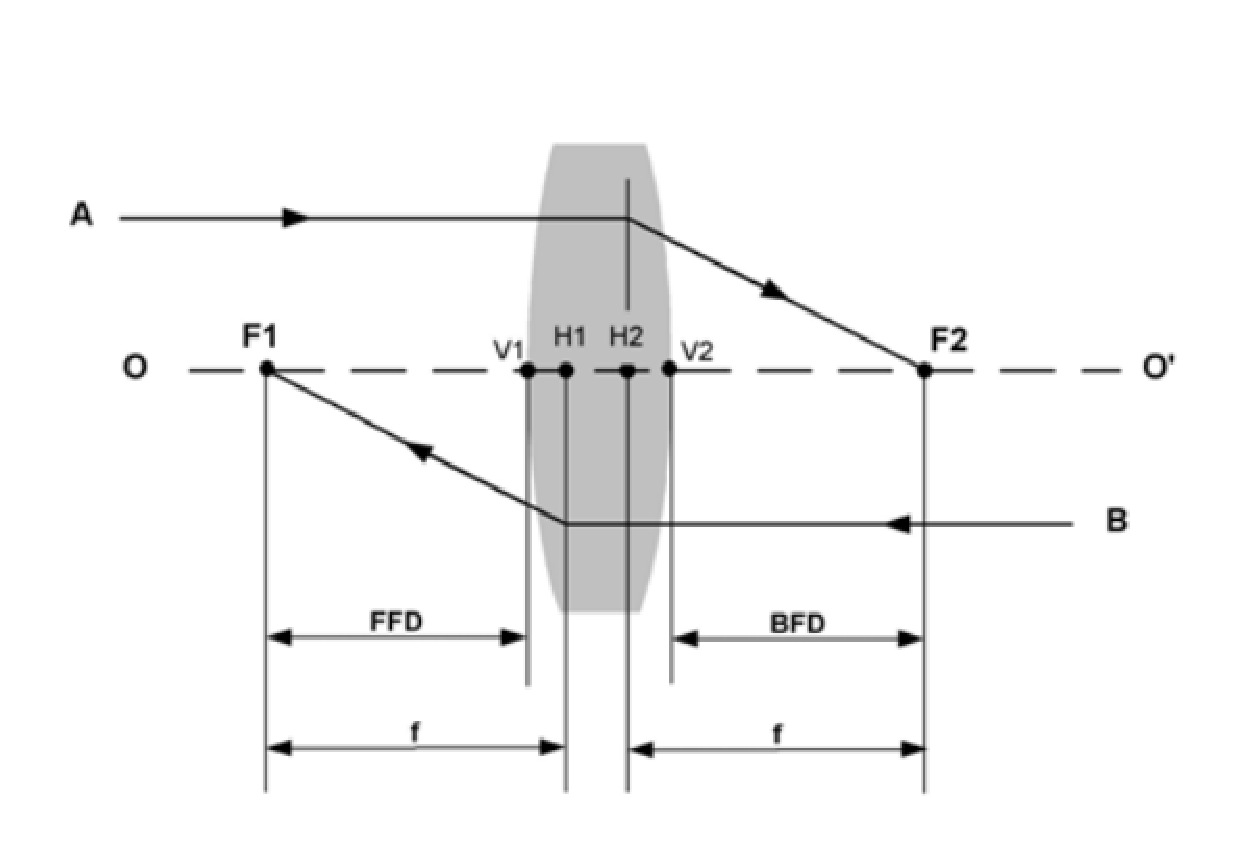
\includegraphics[width=0.33\textwidth]{bilder/lens_define}
\caption{The quantities define of singlet lenses}
\label{fig:lens_define}
\end{figure}

The optical axis (O-O')of the lens is a line passing through the centers of curvature of the two spherical lens surfaces. 
Rays A and B,parallel with the optic axis (O-O'), are  casted from different two sides through the lens and respectively cross the axis at their front and back focal points $F1$ and $F2$. The front and back principal points $H1$ and $H2$ are the intersections of the optical axis with the front and back principal surfaces. Points $V1$ and $V2$ are called the front and back vertices respectively. So important Quantities are defined in the Tab.\ref{tab:lens_quantities}.


\begin{table}
\begin{tabular}{|c|c|c|}
\hline
\textbf{Symbol}&\textbf{Description}&\textbf{Formular}\\
\hline
$f$ & \parbox[c]{6cm}{
						\begin{center}
						effective focal length
						\end{center}
				}& $\frac{1}{f}=(n-1)\left[\frac{1}{R_{1}}-\frac{1}{R_{2}} \right]+\frac{t_{c}(n-1)^2}{nR_{1}R_{2}}$ \\
\hline
$BFD$ &\parbox[c]{6cm}{
						\begin{center}
						back focal distance 
						\end{center}
			}& $BFD=f\left[ 1-\frac{t_{c}(n-1)}{nR_{1}}\right]$ \\
\hline
$FFD$ &\parbox[c]{6cm}{
						\begin{center}
						 front focal distance
						 \end{center} 
			}& $FFD=f\left[ 1+\frac{t_{c}(n-1)}{nR_{1}}\right]$ \\
\hline
$H2V2$ & \parbox[c]{6cm}{
						\begin{center}
						back vertex to back principal point distance
						\end{center}						
			} & $H_{2}V_{2}=f-BFD=-f\frac{t_{c}(n-1)}{nR_{1}}$ \\
\hline
$V1H1$ & \parbox[c]{6cm}{
						\begin{center}			
				    front vertex to front principal point distance
				    \end{center}
				 } & $V_{1}H_{1}=f-FFD=-f\frac{t_{c}(n-1)}{nR_{2}}$ \\
\hline
\end{tabular}
\caption{Important Quantities for Singlet Lenses Immersed in Air}
\label{tab:lens_quantities}
\end{table}


The distance $t_{c}$ is the center thinckness of the lens $V1V2$. 






The classical singlet lenses are plano convex, plano concave, equiconvex and equiconcave lenses, which are listed in following Tab.\ref{tab:lenses_focal_length} with their focal lengths.

\begin{table}
\begin{tabular}{|c|c|c|}
\hline
\textbf{Type}&\textbf{Description}&\textbf{Formular}\\
\hline
Plano Convex & \parbox[c]{2.1cm}{
\includegraphics[width=2cm]{bilder/plano_convex}}& $f=\frac{R}{(n-1)}$ \\
\hline
Plano Concave &\parbox[c]{2.1cm}{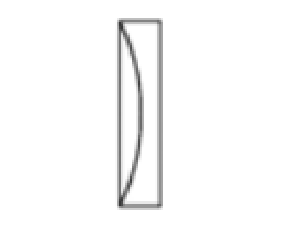
\includegraphics[width=2cm]{bilder/plano_concave}} & $f=-\frac{R}{(n-1)}$ \\
\hline
Equiconvex & \parbox[c]{2.1cm}{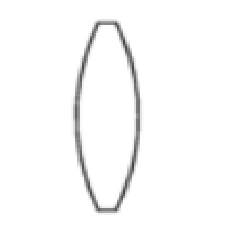
\includegraphics[width=2cm]{bilder/equi_convex}} & $f=\left[\frac{2(n-1)}{R} - \frac{t_{c}(n-1)^2}{nR^2}\right]^{-1}$ \\
\hline
Equiconcave & \parbox[c]{2.1cm}{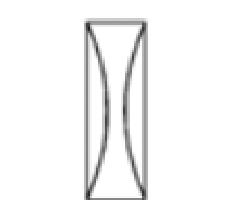
\includegraphics[width=2cm]{bilder/equi_concave}} & $f=\left[\frac{2(n-1)}{R} + \frac{t_{c}(n-1)^2}{nR^2}\right]^{-1}$ \\
\hline
\end{tabular}
\caption{Focal length Formulas of Simple Singlet Lenses in Air.  
				 The Radii are considered positive in the formulas below.}
\label{tab:lenses_focal_length}
\end{table}


High quality singlet lensese are of particular interest in laser focusing and beam handling applications because of their low cost, high damage threshold, and availability of a large variety of standard parts. ..................
	
\subsection{Optical waveguides and Fibers}
%optics
Optical fibers are widely used as a medium for telecommuniction and networking because of varity of advantages.It is flexible,especially permits transmission over longer distances and at higher bandwidths (data rates) than other forms of communication. The Fig.\ref{fig:opticfiber} presents a simplest optical fiber and how lights progate in the fiber. 

\begin{figure}[httbp]
\centering
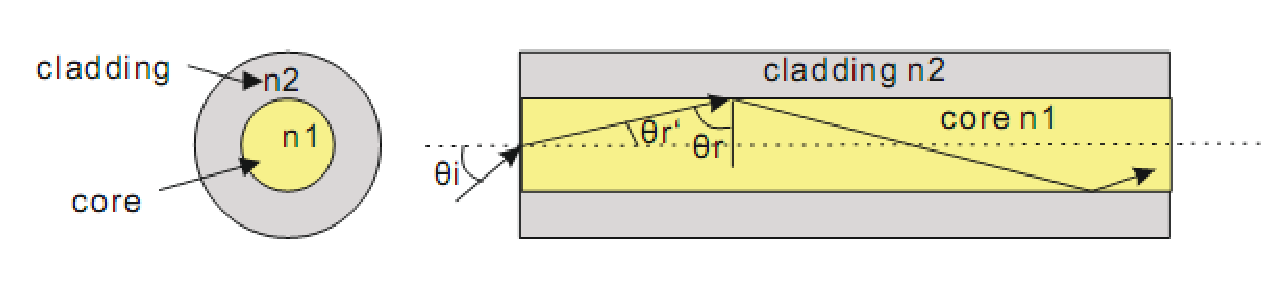
\includegraphics[width=0.8\textwidth]{bilder/opticfiber}
\caption{linght refraction in optic fibers}
\label{fig:opticfiber}
\end{figure}

Optical fiber typically consists of a transparent core with index $n1$ surrounded by a transparent cladding material with a lower index of refraction $n2$. The Light is kept in the core by total internal reflection. This causes the fiber to act as a waveguide.
The principle of the total reflection is explained in \cite{script_FT_TET} with Snell's law. In Fig.\ref{fig:totalreflection} linghts strike a boundary between two different isotropic media with respective refractive indices $n_{1}$ and $n_{2}$ ($n_{1}>n_{2}$), it behaves after Snell's law, which is presented in following mathematical fomular (\ref{eq:snell}).
\begin{figure}[httbp]
\centering
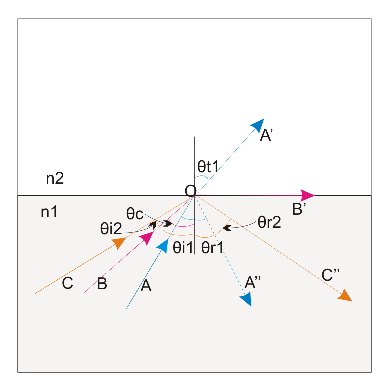
\includegraphics[width=0.6\textwidth]{bilder/totalreflection}
\caption{total reflection}
\label{fig:totalreflection}
\end{figure}

\begin{equation}
n_{1}sin\theta_{i}=n_{2}sin\theta_{t}
\label{eq:snell}
\end{equation}

$\theta_{t}$ is transmission angle or refraction angle.
At a small incidence angle $\theta_{i1}$ a light beam can pass through the boundary and bend to a new course at transmission angle $\theta_{t1}$ in the second meadium.
When the incidence angle is larger than a particular critical angle (\ref{eq:critical_angle}) with respect to the normal to the surface, no light can pass through and all of the light is reflected like (O-C''). In this case the value of $sin\theta_{t}$ in (\ref{eq:sin_transmission_angle}) become larger than one and he mathematical formular of the new transmission angle can be presented by a complex symble $\underline{\theta_{t}}$(\ref{eq:complex_transmission_angle}). $\underline{\theta_{t}}$ is not a real physical angle.

\begin{equation}
\theta_{c}=arcsin(\frac{n_{2}}{n_{1}})
\label{eq:critical_angle}
\end{equation}

\begin{equation}
sin\theta_{t}=\frac{n_{1}}{n_{2}}sin\theta_{i}
\label{eq:sin_transmission_angle}
\end{equation}

\begin{equation}
\underline{\theta_{t}}=\frac{\pi}{2}+j\gamma
\label{eq:complex_transmission_angle}
\end{equation}
with
\begin{equation}
sin\underline{\theta_{t}}=cosh\gamma=\frac{n{1}}{n_{2}}sin\theta_{i},\hspace{2cm}\hfill cos\underline{\theta_{t}}=jsinh\gamma=j\sqrt{cosh^2\gamma-1}
\label{eq:trangle_transmission_angle}
\end{equation}


%Numerical Apertur
Back to the Fig.\ref{fig:opticfiber} the incidence beam originate from the aire into the fiber. There is a maximus coupling angle,so that the beam can be guided under the total reflecting conditions. Its sinus value(\ref{eq:NA}) is called \textbf{Numerical Apertur(NA)}, which indicate the acceptable range of ray beams.

\begin{align}
sin\theta_{i}&=\frac{n_{1}}{n_{0}}sin(90^{o}-\theta_{c})=n_{1}cos\theta_{c} \nonumber\\
&=n_{1}\sqrt{1-sin^{2}\theta_{c}}=n_{1}\sqrt{1-\left(\frac{n_{2}}{n_{1}}\right)^2}=\sqrt{n^2_{1}-n^2_{2}}
\label{eq:NA}
\end{align}


\section{Gaussian Beam}
\label{sect:gaussian_beam}
In nature world there is no source of parallel ray. Each beams of lights can be in some ways considered from a simple origin: point light source,which emits light in all directions. Thus a normal light source can not provide a perfect focused beams for optical applications. Laser light (laser radiation)has some very special properties, which very much distinguish it from light with other origins:

\begin{itemize}
\item Laser light is usually delivered in the form of a laser beam, i.e. it propagates dominantly in a well-defined direction with moderate beam divergence. Such a laser beam has a high (sometimes extremely high) degree of spatial coherence. This means that the electric fields at different locations across a beam profile oscillate with a rigid phase relationship. Exactly this coherence is the reason why a laser beam can propagate over long distances without spreading very much in the transverse directions, and why it can be focused to very small spots (high focusability of laser beams).

\item In many but not all cases, laser light also has a high degree of temporal coherence, which is equivalent to a long coherence length. This means that a rigid phase relationship is also maintained over relatively long time intervals, corresponding to large propagation distances (often many kilometers) or to huge numbers of oscillation cycles.
\item The large temporal coherence, quantified with a large coherence time or coherence length, is associated with a narrow spectral bandwidth (or linewidth). (We exclude here the sophisticated case of trains of ultrashort pulses, which can have a large optical bandwidth but nevertheless a high degree of coherence; see the article on coherence for details.) For a visible laser beam, this means that it has a certain pure color, e.g. red, green or blue, but not white or magenta. Some lasers allow a degree of wavelength tuning (e.g. dye lasers). The large coherence length introduces a tendency for the phenomenon of laser speckle, i.e. a characteristic granular pattern which can be observed e.g. when the laser beam hits a metallic surface.

\item In most cases, laser light is linearly polarized. This means that the electric field oscillates in a particular spatial direction (? polarization of laser emission).
\end{itemize}

Optical engineers and researchers working on optics 


 %light beams where the electric field profile in a plane perpendicular to the beam axis can be described with a Gaussian function, possibly with an added parabolic phase profile
To undersstand the behavior of laser beams in optics system some characteristics are in following  introduced. 

In optics and particularly in laser physics, laser beams often occur in the form of Gaussian beams, which are named after the mathematician and physicist Johann Carl Friedrich Gau�. Here, the transverse profile of the optical intensity of the beam with a power $P$ can be described with a Gaussian function:

\begin{align}
I(r,z)&=\frac{P}{\pi w(z)^2 /2}exp(-2\frac{r^2}{w(z)^2})
\end{align}


where the beam radius w(z) is the distance from the beam axis where the intensity drops to $1/e2 (\sim13.5\%)$ of the maximum value. A hard aperture with radius w can transmit $\sim86.5\%$ of the optical power. For an aperture radius of $1.5 w$ or $2 w$, this fraction is increased to $98.9\%$ and $99.97\%$, respectively.

In addition to the Gaussian shape of the intensity profile, a Gaussian beam has a transverse phase profile which can be described with a polynomial of at most second order. A linear phase variation in one direction (not considered further here) describes a tilt, and a quadratic phase variation is associated with divergence or convergence of the beam.


Gaussian beams are usually considered in situations where the beam divergence is relatively small, so that the so-called paraxial approximation can be applied. This approximation allows the omission of the term with the second-order derivative in the propagation equation (as derived from Maxwell's equations), so that a first-order differential equation results. Within this approximation, a Gaussian beam propagating in free space remains Gaussian, except that of course its parameters evolve. For a monochromatic beam, propagating in the $z$ direction with the wavelength $\lambda$, the complex electric field amplitude (phasor) is
\begin{align}
E(r,z) =E_{0}\frac{w_{0}}{w(z)}exp(-2\frac{r^2}{w(z)^2})exp(-i[kz-arctan\frac{z}{z_{R}}+\frac{kr^2}{2R(z)}])
\end{align}

with the peak amplitude $|E0|$ and beam radius w0 at the beam waist, the wavenumber $k = 2\pi /\lambda$, the Rayleigh length $z_{R}$ (see below) and the radius of curvature $R(z)$ of the wavefronts. The oscillating real electric field is obtained by multiplying the phasor with $exp(i 2\pi ct/ \lambda)$ and taking the real part.

\begin{figure}
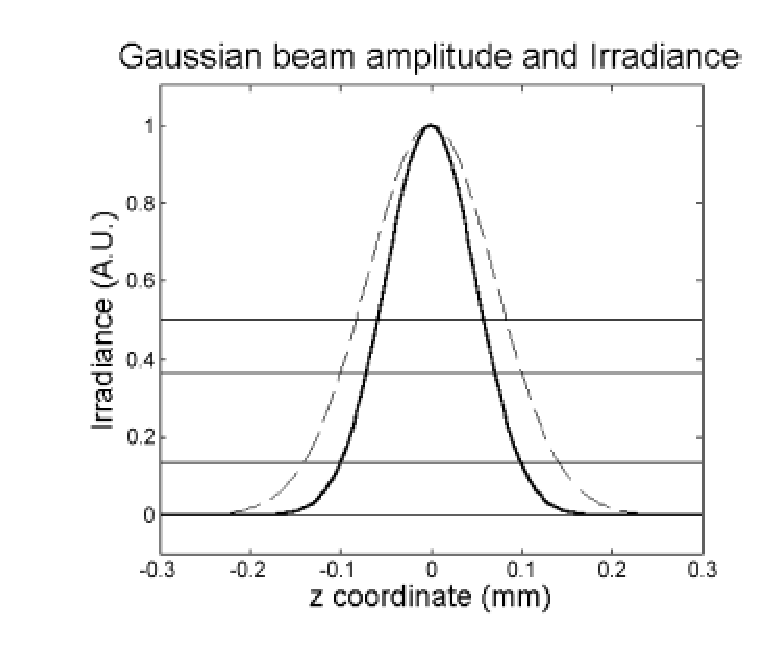
\includegraphics[width=0.8\textwidth]{bilder/gussian_verteilung}
\caption{Transversal profie of the Gussian beam amplitude at the beam waist (dashed line) and irradiance (solid line). Both of them have been normalized to the maximum value. The value of the width of the beam waist $\omega_{0}$ is 0.1 mm. The horizontal lines represent  (in increasing value)the $1/e^{2}$ of the maximum irradiance, the $1/e$ of the maximum amplitude, and the 0.5 of the maximum irrance and amplitude.}
\label{discretization_material}
\end{figure}


\section{Finite Integration Method}
%FIT

%\begin{align}
%%\[
%\oint_{\partial A}\vec{E}\cdot\mathrm{d}\vec{s}=
%-\frac{\mathrm{d}}{\mathrm{d}t}\int_{A}\vec{B}\cdot\mathrm{d}\vec{A}\\
%%\]
%%\\
%%\[
%\oint_{\partial A}\vec{H}\cdot\mathrm{d}\vec{s}=
%\int_{A}(\frac{\partial\vec{D}}{\partial t}+\vec{J})\cdot\mathrm{d}\vec{A}\\
%%\]
%%\\
%%\[
%\oint_{\partial V}\vec{D}\cdot\mathrm{d}\vec{A}=
%\int_{V}\rho\mathrm{d}V\\
%%\]
%%\\
%%\[
%\oint_{\partial V}\vec{B}\cdot\mathrm{d}\vec{A}=0
%%\]
%\end{align}
The Finite Integration Theory(FIT) is a numerical simulation method,which was introduced at 1976 by Thomas Weiland to solving the electromagnetical problems after the Maxwell's functions.

\begin{align}
\oint_{\partial A}\vec{E}\cdot\mathrm{d}\vec{s}&=
-\frac{\mathrm{d}}{\mathrm{d}t}\int_{A}\vec{B}\cdot\mathrm{d}\vec{A}\\
\oint_{\partial A}\vec{H}\cdot\mathrm{d}\vec{s}&=
\int_{A}(\frac{\partial\vec{D}}{\partial t}+\vec{J})\cdot\mathrm{d}\vec{A}\\
\oint_{\partial V}\vec{D}\cdot\mathrm{d}\vec{A}&=
\int_{V}\rho\mathrm{d}V\\
\oint_{\partial V}\vec{B}\cdot\mathrm{d}\vec{A}&=0
\end{align}



%fig: discretization of the material
\begin{figure}
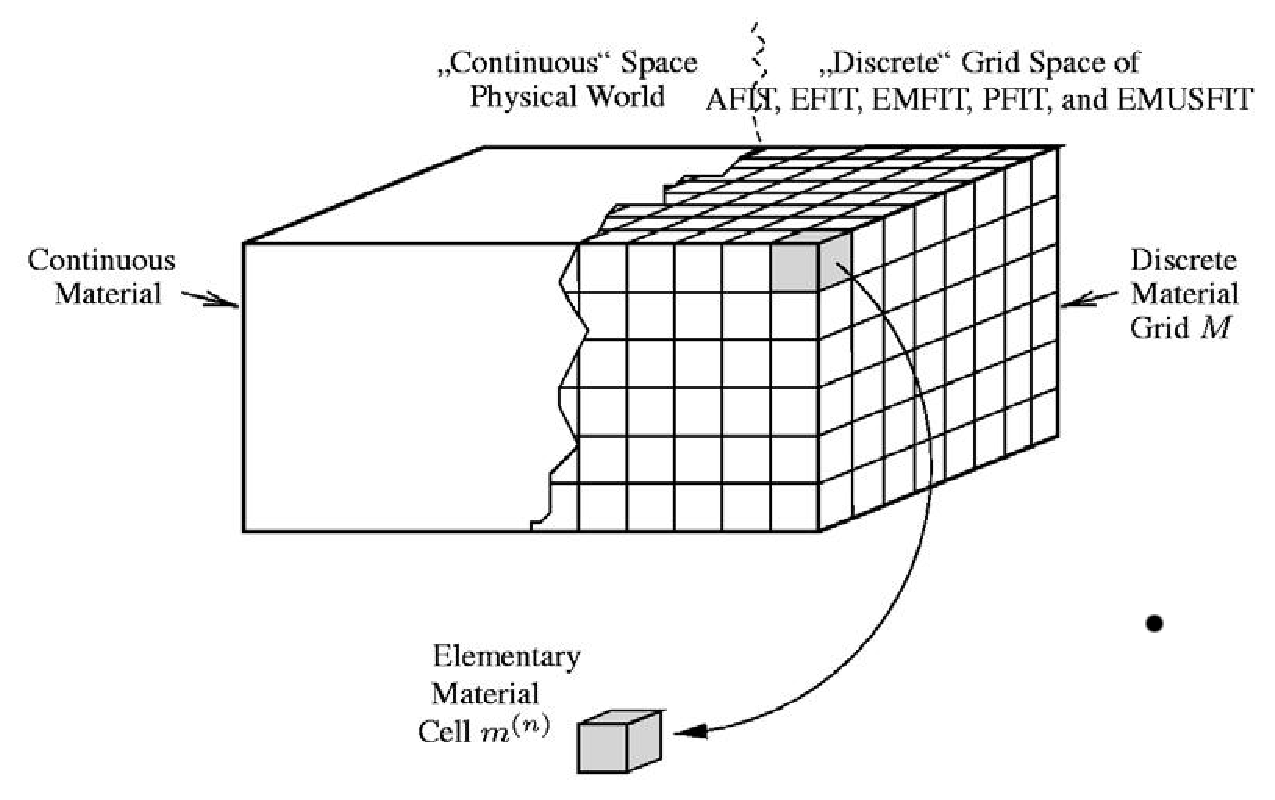
\includegraphics[width=0.8\textwidth]{bilder/discretization_material}
\caption{A discretization of the material in elementary material cells m, defining the material grid M.}
\label{fig:discretization_material}
\end{figure}



%%law inductive

Following is a demonstration of the discretized form from the inductive law (\ref{eq:maxwell_1}). Considering the path integral in a single element edge like Fig.  \ref{fig:FIT_max_integral1}, the left side of (\ref{eq:maxwell_1}) can be presented as  (\ref{eq:inductive_left}). 

\begin{figure}[!ht]
\centering
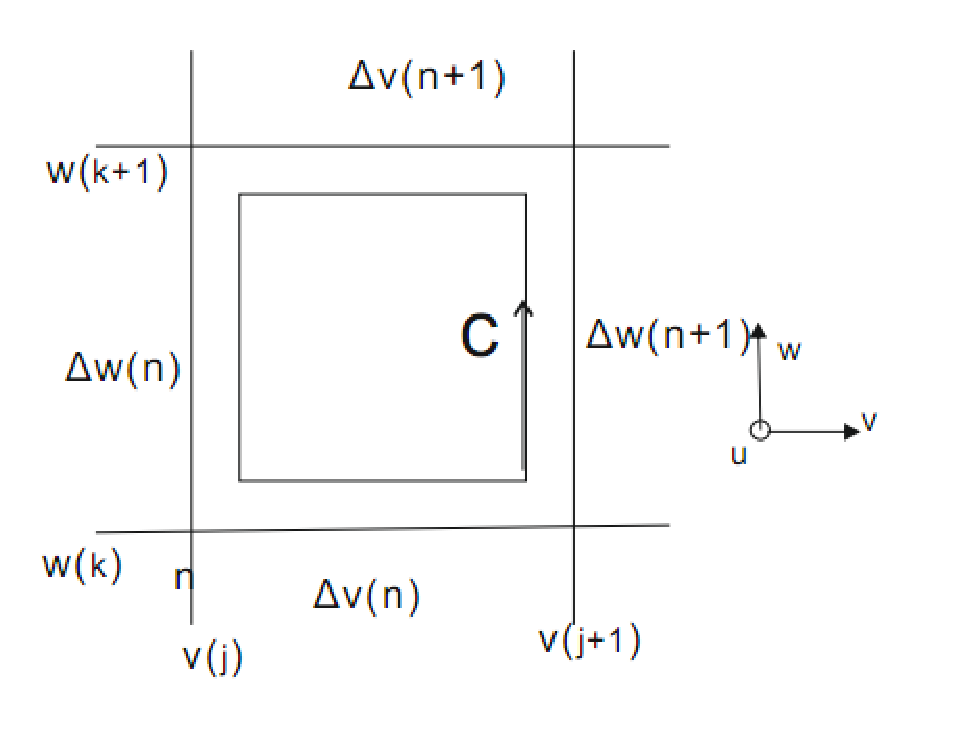
\includegraphics[width=0.45\textwidth]{bilder/FIT_max_integral1}
\caption{ Path integral along edges of one single elemental plane $A_{u}(n)$\cite{ script_FeldSim}.}
\label{fig:FIT_max_integral1}
\end{figure}

\begin{figure}[!ht]
\centering
\subfigure[Discrete electric field strength components distribute at edges of grids.]{
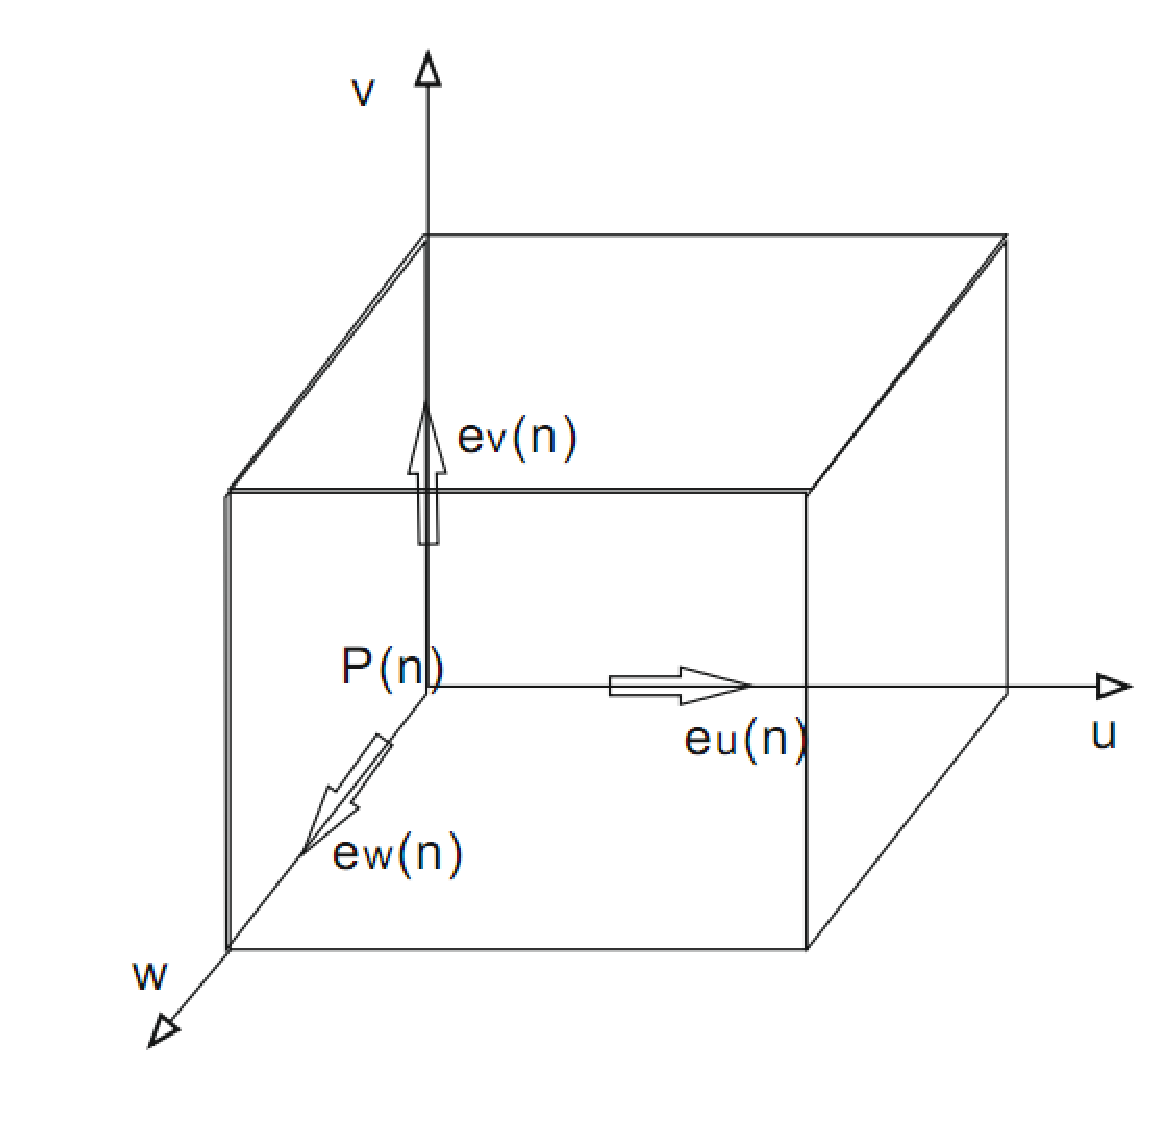
\includegraphics[width=0.4\textwidth]{bilder/FIT_max_integral2}
\label{fig:FIT_max_integral2}
}
\hfill
\subfigure[Discrete magnetic flux density components distribute at planes of grids.]{
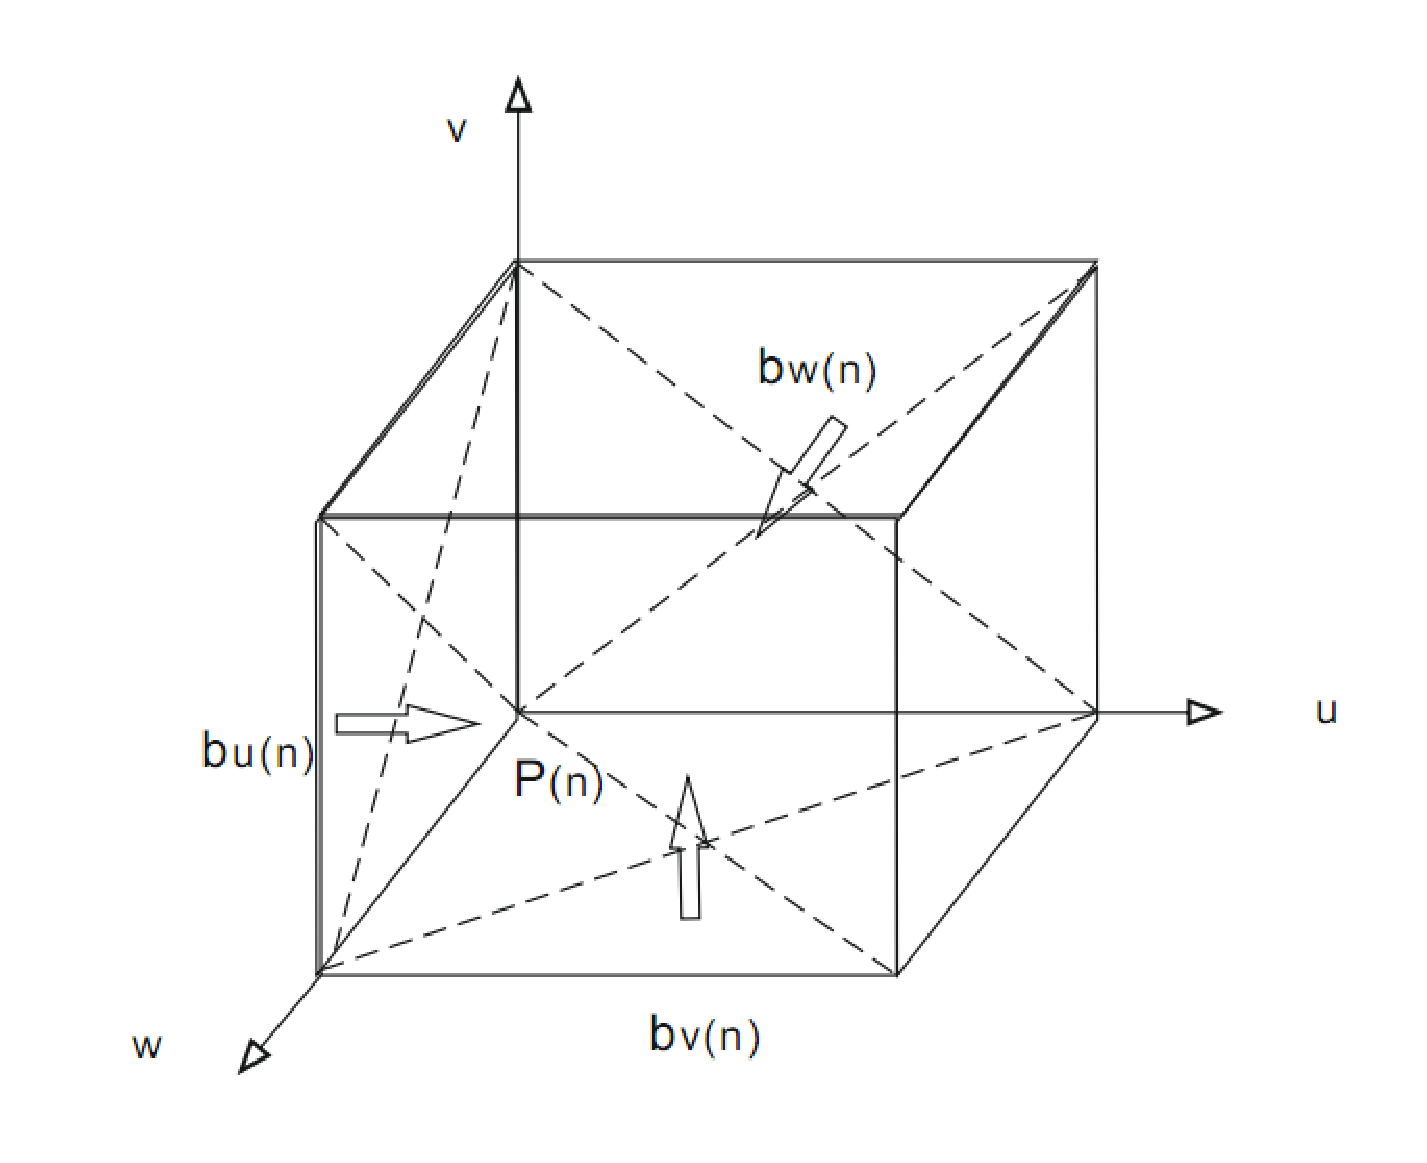
\includegraphics[width=0.5\textwidth]{bilder/FIT_max_integral3}
\label{fig:FIT_max_integral3}
}
\caption{Allocations of components at grids\cite{ script_FeldSim}.}
\end{figure}

\begin{equation}
\int_{C}\vec{E}\cdot d\vec{s}
=\underbrace{\int_{\Delta v(n)}\vec{E}\cdot d\vec{s}}_{\se_{v}(n)}
+\underbrace{\int_{\Delta w(n+M_{v})}\vec{E}\cdot d\vec{s}}_{\se_{w}(n+M_{v})}
-\underbrace{\int_{\Delta v(n+M_{w})}\vec{E}\cdot d\vec{s}}_{\se_{v}(n+M_{w})}
-\underbrace{\int_{\Delta w(n)}\vec{E}\cdot d\vec{s}}_{\se_{w}(n)}
\label{eq:inductive_left}
\end{equation}

Where $\widehat{e}(n)$ is so called  electric grid voltage and has the following relation with electric field strength $e(n)$ (seeing Fig. \ref{fig:FIT_max_integral2})
\begin{equation}
 e_{v}(n)=\frac{\se_{v}(n)}{\Delta v(n)}
\label{eq:e_field}
\end{equation}
Meanwhile the right hand side of (\ref{eq:maxwell_1}) approximates to (\ref{eq:inductive_right})
\begin{equation}
-\iint_{A_{u}(n)}\frac{\partial\vec{B}}{\partial t}\cdot\mathrm{d}\vec{A} 
=-\iint_{A_{u}(n)}\frac{\partial B^{*}_{u}}{\partial t}\cdot\mathrm{d}A
\approx -\frac{\partial}{\partial t}b_{u}(n)A_{u}(n)
\label{eq:inductive_right}
\end{equation}
Where $A_{u}(n)=\Delta v(n)\Delta w(n)$ and $b_{u}(n)$ (Fig. \ref{fig:FIT_max_integral3}) is magnetic flux density, given by
\begin{equation}
 b_{u}(n)=\frac{\widehat{\widehat{b}}_{u}(n)}{\Delta A_{u}(n)} \text{,}
\label{eq:b_flux_density}
\end{equation}
 and magnetic grid flux $\widehat{\widehat{b}}_{u}(n)$, given by
\begin{equation}
\widehat{\widehat{b}}_{u}(n)=\iint_{A_{u}(n)}\vec{B}\cdot\mathrm{d}\vec{A} \text{.}
\label{eq:mag_fluxe}
\end{equation}
From equations (\ref{eq:inductive_left}-\ref{eq:mag_fluxe}) we obtain the difference form (\ref{eq:inductive_integral}) of the inductive equation at one single elemental plane:
\begin{equation}
\widehat{e}_{v}(n)+\widehat{e}_{w}(n+M_{v})-\widehat{e}_{v}(n+M_{w})-\widehat{e}_{w}(n)=-\frac{\partial}{\partial t}\widehat{\widehat{b}}_{u}(n)
\label{eq:inductive_integral}
\end{equation}
i.e.,
\begin{align}
\Delta v(n)e_{v}(n)&+\Delta w(n+M_{v})e_{w}(n+M_{v})\nonumber\\
-\Delta v(n+M_{w})e_{v}(n+M_{w})&-\Delta w(n)e_{w}(n)=-A_{u}(n)\frac{\partial}{\partial{t}}b_{u}(n) 
\label{eq:inductive_sample}
\end{align}
By merging electric field-strength $e(n)$ and magnetic flux density $b(n)$ of all grids into vectors we obtain
\begin{equation*}
e_{u}:=
\begin{pmatrix}
e_{u}(1)&\\
\vdots&\\
e_{u}(N_{p})&
\end{pmatrix},
e_{v}:=
\begin{pmatrix}
e_{v}(1)&\\
\vdots&\\
e_{v}(N_{p})&
\end{pmatrix},
e_{w}:=
\begin{pmatrix}
e_{w}(1)&\\
\vdots&\\
e_{w}(N_{p})&
\end{pmatrix},
e:=
\begin{pmatrix}
e_{u}&\\
e_{v}&\\
e_{w}&
\end{pmatrix},
\label{eq:vector_e_field}
\end{equation*}
\begin{equation*}
b_{u}:=
\begin{pmatrix}
b_{u}(1)&\\
\vdots&\\
b_{u}(N_{p})&
\end{pmatrix},
b_{v}:=
\begin{pmatrix}
b_{v}(1)&\\
\vdots&\\
b_{v}(N_{p})&
\end{pmatrix},
b_{w}:=
\begin{pmatrix}
b_{w}(1)&\\
\vdots&\\
b_{w}(N_{p})&
\end{pmatrix},
b:=
\begin{pmatrix}
b_{u}&\\
b_{v}&\\
b_{w}&
\end{pmatrix}.
\label{eq:vector_m_flux_density}
\end{equation*}
Expanding the relation (\ref{eq:inductive_sample}) to all grid cells \cite{FIT_discrete_method,FIT_discrete_electrommagnetism} we arrive at the discrete form of inductive equation:
\begin{equation}
CD_{s}e=-D_{A}\frac{\partial}{\partial{t}}b
\label{eq:inductive_sample_all}
\end{equation}
Where $D_{s}$ is elemental edge matrix, given by
\begin{align*}
D_{s}=
%	\begin{pmatrix}
%	\Delta u(1)&&&&&&&&\\
%	&\ddots &&&&&&&\\
%	&&\Delta u(N_{p})&&&&&&\\
%	&&&\Delta v(1)&&&&&\\
%	&&&&\ddots &&&&\\
%	&&&&&\Delta v(N_{p})&&&\\
%	&&&&&&\Delta w(1)&&\\
%	&&&&&&&\ddots &\\
%	&&&&&&&&\Delta w(N_{p})
%	\end{pmatrix}
Diag\{&\Delta u(1),\cdots,\Delta u(N_{p}),\nonumber\\
			&\Delta v(1),\cdots,\Delta v(N_{p}),\nonumber\\
			&\Delta w(1),\cdots,\Delta w(N_{p})
\} \text{.}
	%\label{eq:Ds_matrix}
\end{align*}
$D_{A}$ is elemental plane matrix, given by
\begin{align*}
D_{A}=
%	\begin{pmatrix}
%	\Delta A_{u}(1)&&&&&&&&\\
%	&\ddots &&&&&&&\\
%	&&\Delta A_{u}(N_{p})&&&&&&\\
%	&&&\Delta A_{v}(1)&&&&&\\
%	&&&&\ddots &&&&\\
%	&&&&&\Delta A_{v}(N_{p})&&&\\
%	&&&&&&\Delta A_{w}(1)&&\\
%	&&&&&&&\ddots &\\
%	&&&&&&&&\Delta A_{w}(N_{p})
%	\end{pmatrix}
Diag\{&\Delta A_{u}(1),\cdots,\Delta A_{u}(N_{p}),\nonumber\\
			&\Delta A_{v}(1),\cdots,\Delta A_{v}(N_{p}),\nonumber\\
			&\Delta A_{w}(1),\cdots,\Delta A_{w}(N_{p})
\} \text{.}
	%\label{eq:Da_matrix}
\end{align*}
$C$ is \textbf{curl} operator, given by
\begin{equation*}
C=
	\begin{pmatrix}
	0&-P_{w}&P_{v}\\
	P_{w}&0&-P_{u}\\
	-P_{v}&P_{u}&0
	\end{pmatrix} \text{.}
%\label{eq:C_matrix}
\end{equation*}
\begin{figure}[!ht]
\centering
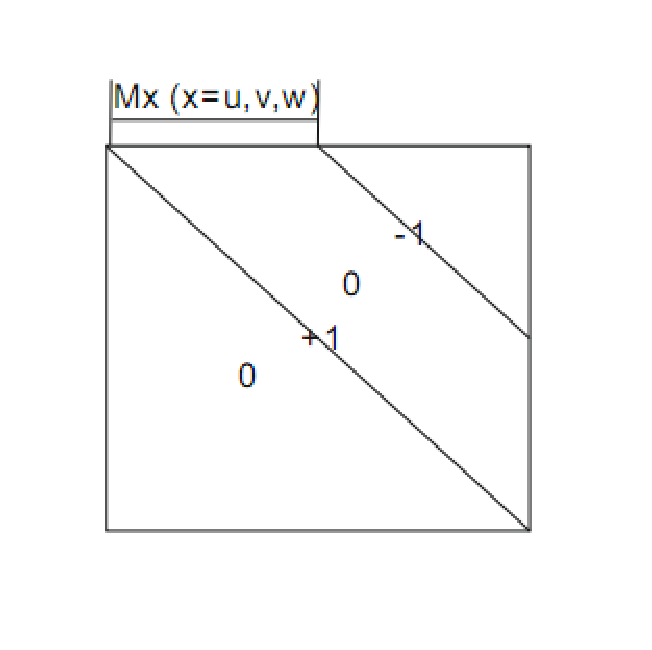
\includegraphics[width=0.35\textwidth]{bilder/P_matrix}
\caption{Structure of matrix $P_{x},(x=u,v,w)$.}
\label{fig:Matrix Px}
\end{figure}
Submatrices $P_{u},P_{v},P_{w}$ are composed of $1,-1,0$ like Fig. \ref{fig:Matrix Px}.\\
 
Alternative form of the equation (\ref{eq:inductive_sample_all}) is given in (\ref{eq:inductive_integral_all})
\begin{equation}
C\widehat{e}=-\frac{\partial}{\partial{t}}\widehat{\widehat{b}}
\label{eq:inductive_integral_all}
\end{equation}
%\widehat{e}
Where $\widehat{e}$ is electric voltage and $\widehat{\widehat{b}}$ magnetic flux.
%divergence equation
Analogy the divergence equation (\ref{eq:maxwell_4}) can also be discretized in grid $G$ and its difference form is given by 
\begin{equation*}
SD_{A}b=0
\label{eq:divergence_sample}
\end{equation*}
or
\begin{equation*}
S\widehat{\widehat{b}}=0
\label{eq:divergence_integral}
\end{equation*}
$S\in \mathbb{R}^{N_{p}\times 3N_{p}}$ represent the discrete divergence matrix, which depends on the grid topology just as the discrete $curl-Matrix$ $C$.
%S
\begin{equation*}
S=(P_{u}|P_{v}|P_{w})
\label{eq:S_matrix}
\end{equation*}
%Amp\'ere's law
For discretizing Amp\'ere's law (\ref{eq:maxwell_2}) \textbf{Dual Grid} is defined, seeing Fig. \ref{fig:dual_grid}. 

\begin{figure}[!ht]
\centering
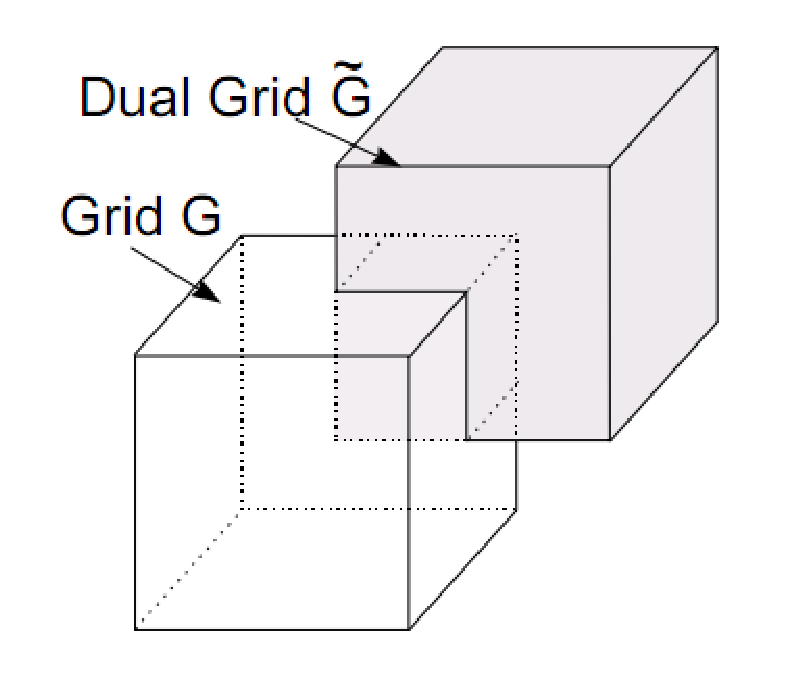
\includegraphics[width=0.5\textwidth]{bilder/dual_grid}
\caption{The allocation of the Primary Grid $G$ and Dual Grid $\tilde{G}$\cite{FIT_discrete_electrommagnetism}.}
\label{fig:dual_grid}
\end{figure}
Then the discretized form of (\ref{eq:maxwell_2}) in dual grid is obtained like
\begin{equation*}
\tilde{C}\tilde{D}_{s}D_{\mu^{-1}}b=\tilde{D}_{A}(D_{\epsilon}\frac{\mathrm{d}}{\mathrm{dt}}e+D_{\kappa}e+j)
\label{eq:ampere}
\end{equation*}
or
\begin{equation*}
\tilde{C}\widehat{h}=\frac{\mathrm{d}}{\mathrm{dt}}\widehat{\widehat{d}}+\widehat{\widehat{j}}_{L}+\widehat{\widehat{j}}_{S}
\label{eq:ampere_sample}
\end{equation*}

Where $\bar{\epsilon}$ is average dielectric constant. $ D_{\epsilon}$ is the average dielectric matrix. $\tilde{C}$ represents the $curl-operator$ in dual grid.
With the help of dual grid cells Gauss' law (\ref{eq:maxwell_3}) in integral form can be discretized\cite{script_FeldSim} as following:
\begin{equation*}
\tilde{S}\widehat{\widehat{d}}=q
\label{eq:gausslaw}
\end{equation*}
or
\begin{equation*}
\tilde{S}\tilde{D}_{A}D_{\epsilon}e=\tilde{D}_{V}\rho_{D}
\label{eq:gausslaw_sample}
\end{equation*}
Where $\rho_{D}$ is the vector of the charge density in grid cells.

\begin{equation*}
\tilde{S}=(\tilde{P}_{u}|\tilde{P}_{v}|\tilde{P}_{w})=(-P_{u}^{T}|-P_{v}^{T}|\-P_{w}^{T})
\label{eq:dual_S_matrix}
\end{equation*}

%fundamental

\section{S-Parmeters}
%S_parameter
Normally an electrical network can be considered as a 'black box', which contains amounts of interconnected basic electrical circuit components such as resistors, capacitors, inductors and transistors etc. On this 'black box' may exist many ports, which present the entries or exits of the network. In order describe the characteristics of this network H-Parameters are used, which describe the relation between voltages and currents. In Fig. \ref{fig:2_port_network} is a 2-port network $V_{1}$ and $V_{2}$ are total voltages of both ports; $I_{1}$ and $I_{2}$ are total currents of both ports respectively. Relations between voltages and currents are like (\ref{eq:voltage_current}). 
\begin{figure}[!ht]
\centering
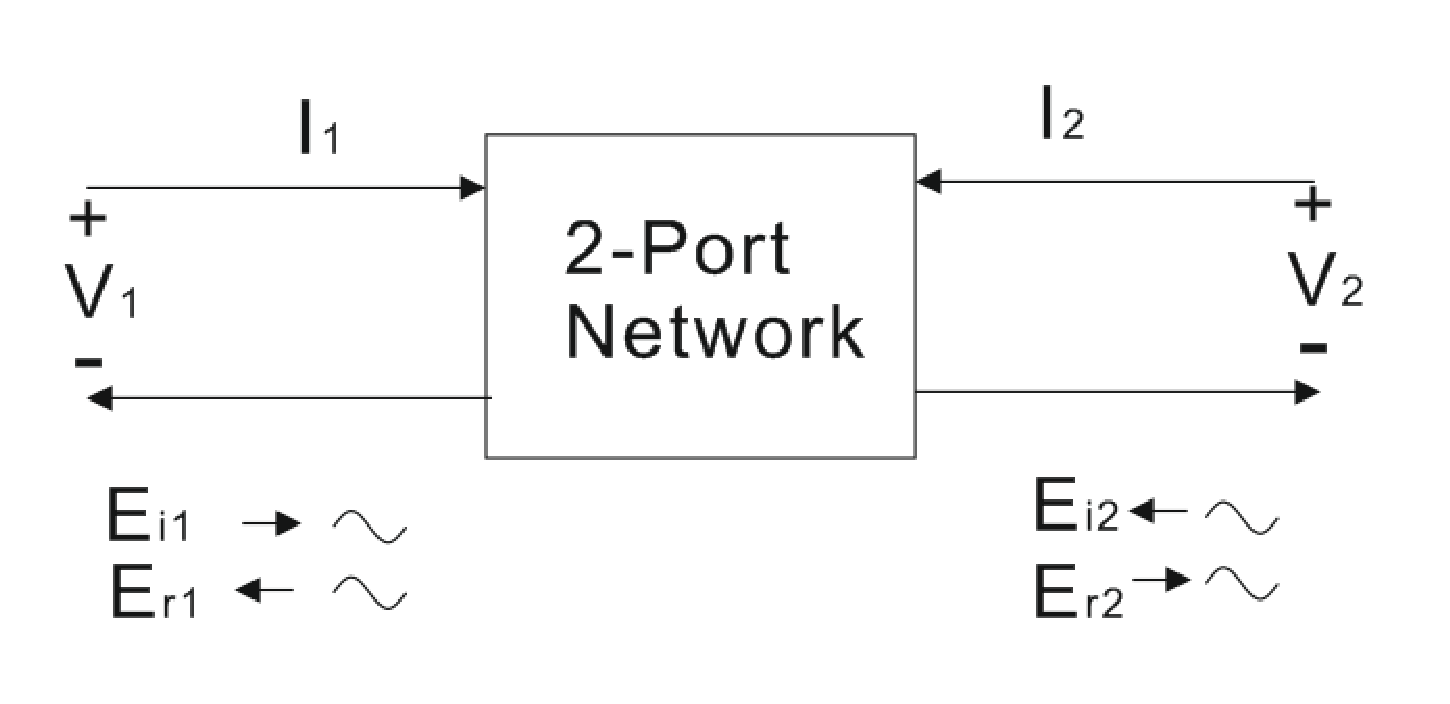
\includegraphics[width=0.6\textwidth]{bilder/s_parameters}
\caption{2-Port-Network \cite{aglient_s_parameters}}
\label{fig:2_port_network}
\end{figure}

\begin{align}
V_{1}&=h_{11}I_{1}+h_{12}V_{2}\\
I_{2}&=h_{21}I_{1}+h_{22}V_{2}
\label{eq:voltage_current}
\end{align}
Where $h_{11},h_{12},h_{21}$ and $h_{22}$ are H-Parameters and defined in (\ref{eq:h_parameters1}-\ref{eq:h_parameters2}).
\begin{align}
h_{11}&=\frac{V_{1}}{I_{1}}|_{V_{2}=0}\quad h_{12}=\frac{V_{1}}{V_{2}}|_{I_{1}=0}
\label{eq:h_parameters1}\\
h_{21}&=\frac{I_{2}}{I_{1}}|_{V_{2}=0}\quad h_{22}=\frac{I_{2}}{V_{2}}|_{I_{1}=0}
\label{eq:h_parameters2}
\end{align}
But H-Parameters cannot always be valid for the description of microwave circuits. Agilent\cite{aglient_s_parameters} has listed some problems of H-Parameters in high frequency:
\begin{itemize}
\item It is not easy to measure the total voltage and total current at the ports of the network.
\item Short and open circuits are not always available for a broad frequency band.
\item For high frequency some circuit are not stable in short or open conditions.
\end{itemize}
Scattering parameters or S-parameters are perfect description of microwave circuit\cite{RF194_s_parameters}. In that case traveling waves are applied instead of total voltages and currents. $E_{i1}$ and $E_{i2}$ represent incidence waves over left and right ports of the network respectively. $E_{r1}$ and $E_{r2}$ are reflective waves. The relation between traveling waves, total voltages and curents has relations (\ref{eq:voltage_wave1}-\ref{eq:voltage_wave2}).
\begin{align}
V_{1}&=E_{i1}+E_{r1}\quad V_{2}=E_{i2}+E_{r2}
\label{eq:voltage_wave1}\\
I_{1}&=\frac{E_{i1}-E_{r1}}{Z_{0}}\quad I_{2}=\frac{E_{i2}-E_{r2}}{Z_{0}}
\label{eq:voltage_wave2}
\end{align}
Traveling waves themselves can be expressed in terms of H-Parameters (\ref{eq:er1}\ref{eq:er2}). 
\begin{align}
E_{r1}&=f_{11}(h)E_{i1}+f_{12}(h)E_{i2}
\label{eq:er1}
\\
E_{r2}&=f_{21}(h)E_{i1}+f_{22}(h)E_{i2}
\label{eq:er2}
\end{align}
Here $f11, f12, f21, f22$ are the network parameters, which indicate the relation between traveling voltages waves and total voltages or currents. Divide both sides of the functions(\ref{eq:er1}-\ref{eq:er2}) by $\sqrt{Z_{0}}$( $Z_{0}$ system impedance).A new set of variables are defined:
\begin{align} 
a1&=\frac{Ei1}{\sqrt{Z_{0}}}=\frac{V_{1}+I_{1}Z_{0}}{2\sqrt{Z_{0}}} \quad a2=\frac{Ei2}{\sqrt{Z_{0}}}=\frac{V_{2}+I_{2}Z_{0}}{2\sqrt{Z_{0}}} \\
b1&=\frac{Er1}{\sqrt{Z_{0}}}=\frac{V_{1}-I_{1}Z_{0}}{2\sqrt{Z_{0}}}  \quad b2=\frac{Er2}{\sqrt{Z_{0}}}=\frac{V_{2}-I_{2}Z_{0}}{2\sqrt{Z_{0}}}
\end{align}
So relations of the new variables are give by:
\begin{align}
b_{1}&=S_{11}a_{1}+S_{12}a_{2}\\
b_{2}&=S_{21}a_{1}+S_{22}a_{2}
\end{align}
or in matrics form:
\begin{equation}
		\begin{pmatrix}
			b_{1}&\\
			b_{2}&
		\end{pmatrix}
	=	
		\begin{pmatrix}
			S_{11}&S_{12}\\
			S_{21}&S_{22}
		\end{pmatrix}
		\begin{pmatrix}
			a_{1}&\\
			a_{2}&
		\end{pmatrix}
\label{eq:s_matrix}
\end{equation}

The S-Parameters are defined as following:
\begin{align}
S_{11}&=\frac{b_{1}}{a_{1}}|_{a_{2}=0}\\
S_{21}&=\frac{b_{2}}{a_{1}}|_{a_{2}=0}\\
S_{22}&=\frac{b_{2}}{a_{2}}|_{a_{1}=0}\\
S_{12}&=\frac{b_{1}}{a_{2}}|_{a_{1}=0}
\end{align}
The phical meaning of the S-Parameters are described as following:
\begin{itemize}
\item $S_{11}$ is the input port reflection coefficient
\item $S_{12}$ is the reverse gain
\item $S_{21}$ is the forward gain
\item $S_{22}$ is the output port reflection coefficient
\end{itemize}
In another hand, $S_{21}$ is often used to estimate the transmission ability of a network. Therefore $S_{21}$ equals the coupling efficiency in this work.


\chapter{Modelling}
\label{chp:model}
%Chapter2
%description

In this chapter the configurations of the experimental objects and corresponding technical detail will be at first introduced. Then it will be described the detail how the simulation models are approximated in CST MWS (CST Studio suite 2010) and the some performances of the simulations will also be illustrated in compare with the practical objects, such as working distance, minimum spot size, power distribution, etc .

\section{Project description}

%Project description
% Problem description
Coupling single-mode fibers to waveguides (Fiber-to-Chip coupling) by microlenses is a very common problem in integrated optics \cite{ integrated_optics}, in wich waveguides locate on a substrate. By means of this technology the simple and reliable optical system with a small size become possible because a lensed fiber has a minized focal length. In this works the application of the lensed fiber-to-chip will be introduced and it coupling efficiency will be discussed.\\
Fig. \ref{fig:experiment_object} is a schematic demonstration of fiber-to-chip coupling. At the one side there is a lensed tapered fiber as laser source and at another side at the working distance of the fiber there is a buried rib waveguide\cite{integrated_optics} as signal receiver. The purpose of this works is to find a way to gain optimized coupling efficiency through the simulations in CST MWS, which is a electromagnetic simulator basically with the implementation of the Finite Integration Technique (FIT)\cite{cst_help_siulation_method}. 


\begin{figure}[!ht]
\centering
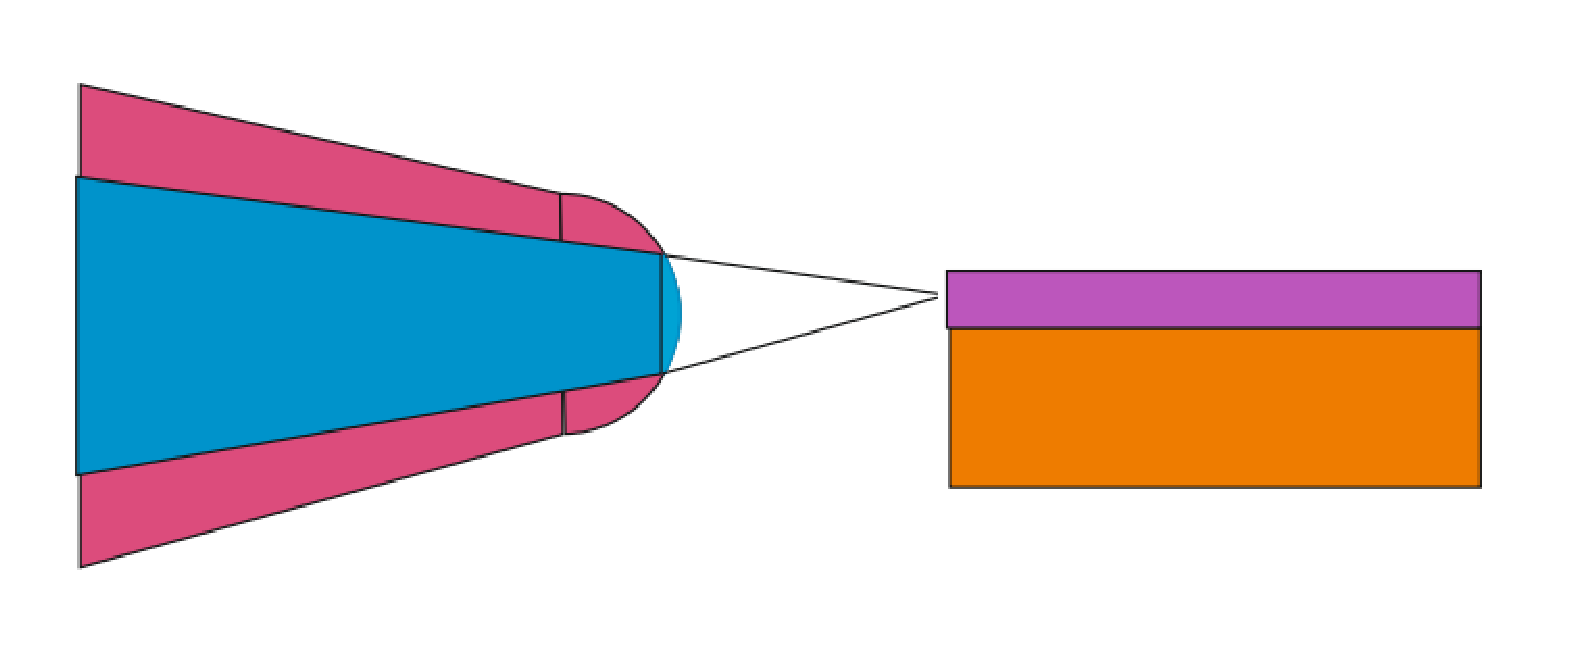
\includegraphics[width=.7\textwidth]{bilder/experiment_object}
\caption{Fiber-to-Chip Coupling}
\label{fig:experiment_object}
\end{figure}

\begin{figure}[!ht]
\centering
\subfigure[Picture of a real Single mode lensed fiber\cite{nanoscal_tapered_fiber}.]{
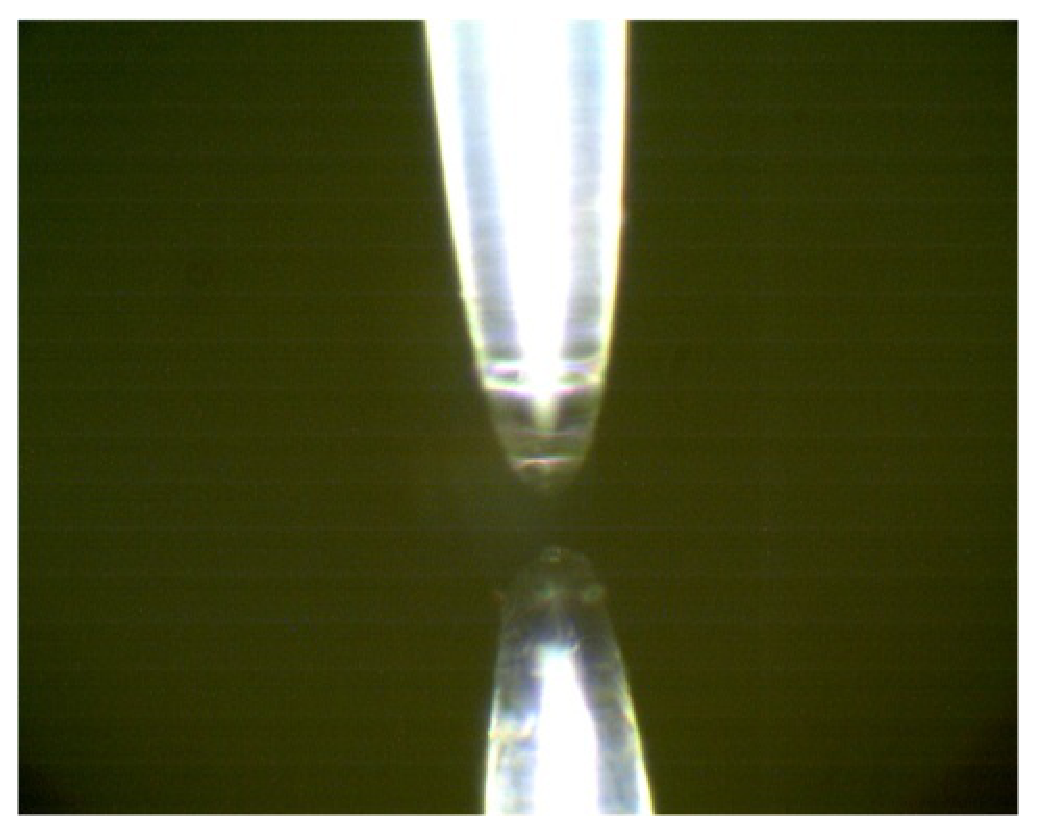
\includegraphics[width=0.3\textwidth]{bilder/single_mode_lensed_fibber}
\label{fig:single_mode_lensed_fiber}
}
\hfill
\subfigure[Schema of a tapered lensed fiber\cite{nanoscal_tapered_fiber}.]{
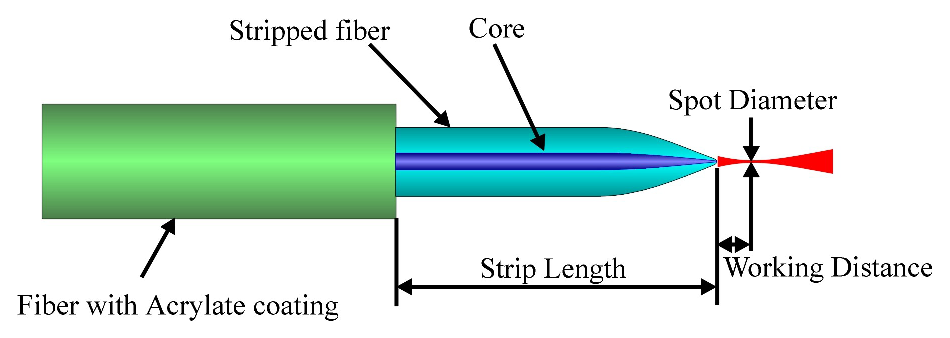
\includegraphics[width=0.6\textwidth]{bilder/tapered_lensed_fiber}
\label{fig:tapered_lensed_fiber}
}
\label{fig:TLFs}
\caption{NANOICS Tapered and Lensed Fibers}
\end{figure}


In this works the the tapered lensed fiber from NANONICS\cite{nanoscal_tapered_fiber} will be used. Fig.\quad\ref{fig:single_mode_lensed_fiber} is the real image of the fiber and Fig.\quad\ref{fig:tapered_lensed_fiber} indicate its schema. In Tab.\quad\ref{tab:technical parameters_lensed_fiber} are listed part of technical parameters, which refer later to the modeling. Additionally the real woking frequence is $\lambda=1064$nm and working distance but $4\mu$m. 
\begin{table}
\caption{Technical parameters about tapered lensed fiber.\cite{nanoscal_tapered_fiber}}
\begin{tabular}{c|c|c}
\hline
\multicolumn{2}{c|}{\textbf{Parameter}}&\textbf{Specification(Single-Mode)}\\
\hline
\multirow{3}{*}{\parbox[t]{0.25\textwidth}{Spot Size of Aspheric and Convex Lenses($1/e^2$)}}&\multirow{2}{*}{Minum}&$1.7\mu$m($\lambda=1.5\mu$m)\\
&																		 &$0.6\mu$m($\lambda=0.6\mu$m)\\
\cline{2-3}
&Maxium															 &$6.0\mu$m($\lambda=1.5\mu$m)\\
\hline
\multirow{2}{*}{Spot Size Tolerance}&\parbox[t]{0.25\textwidth}{Without near-field characterization} &$\pm 0.5\mu$m\\
\cline{2-3}
&\parbox[t]{0.25\textwidth}{With near-field characterization} &$\pm 0.25\mu$m\\
\hline
\multirow{2}{*}{Working Distance} &Minimum &$5\mu$ m($\lambda=1.5\mu$m)\\
\cline{2-3}
&																	Maximum &$50\mu$ m($\lambda=1.5\mu$m)\\
\hline
\end {tabular}

\label{tab:technical parameters_lensed_fiber}
\end{table}

\begin{figure}
\centering
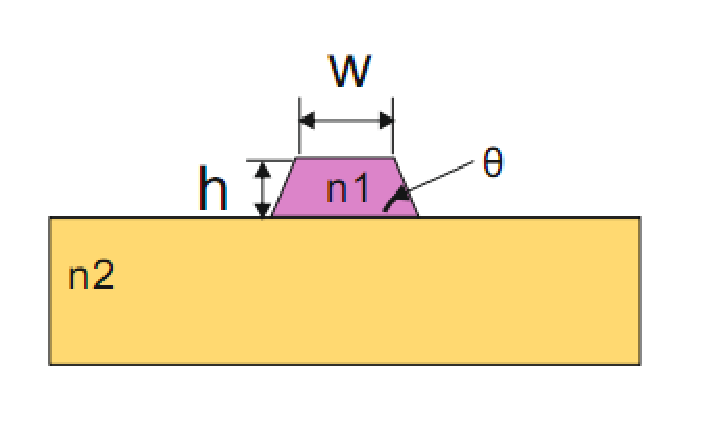
\includegraphics[width=0.4\textwidth]{bilder/orignial_waveguide}
%\subfigure[Schema of a real waveguide.]{
%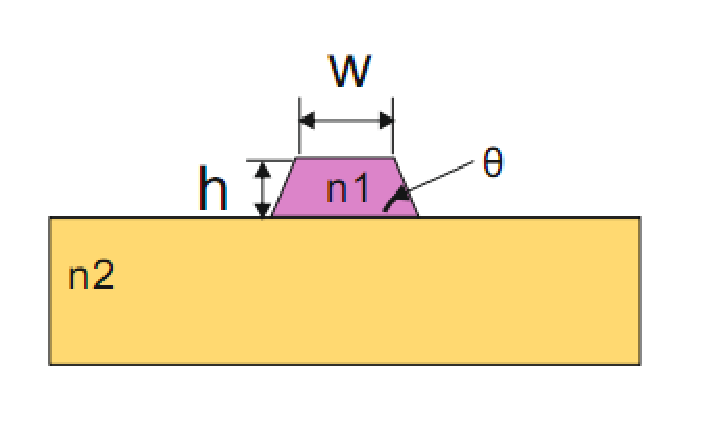
\includegraphics[width=0.4\textwidth]{bilder/orignial_waveguide}
%\label{fig:orignial_waveguide}
%}
%\hfill
%\subfigure[Schema of a approxmate waveguide.]{
%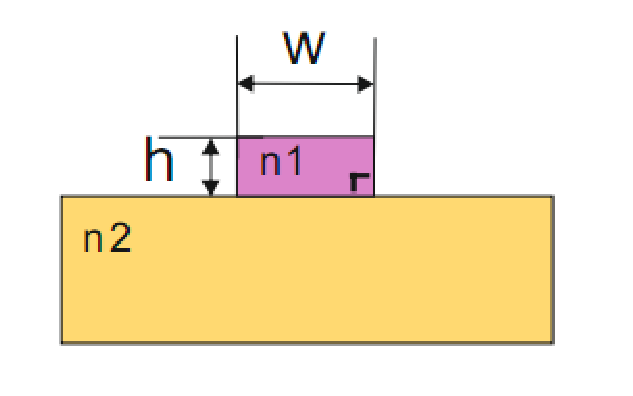
\includegraphics[width=0.4\textwidth]{bilder/approxmate_waveguide}
%\label{fig:approxmate_waveguide}
%}
\caption{Schema of the photonic waveguide}
\label{fig:photonic_waveguide}
\end{figure}
The practical waveguide Fig. \ref{fig:orignial_waveguide} is a trapezoid guide on a semiconductor. But the angles $\theta$ of this guide approximate to $90^{o}$ and is not easy to measure because of its micro-size. Thus a simplified guide model Fig.\ref{fig:approxmate_waveguide} will be used in this works. And the detailed technical properties of the photonic waveguide are given:
\begin{itemize}
\item Working frequency: $\lambda=1064\mu$m
\item Waveguide: LiNbO$_{3}$ with $n_{1}=2.516, w\approx 1\mu$m, $h\approx 0.5 \mu$m
\item Substrate: SiO$_{2}$ with $n_{2}=1.544 $
\end{itemize}

\section{Modelling and Simulation}
\label{sect:model_simulation}
%modeling_introduction
For an economic simulation there is no need to create exactly identical models.  Sometimes only parts of the specifics are requested. In this section the modeling process will be discussed. 
\subsection{Modelling the Lensed Fiber}
\label{sect:model_model_model_TLF}
%fiber_modeling

%\section{Modeling the Lensed Fiber}

Firstly, it is demanded to determine the Tapered and Lensed Fiber(TLF) model. Because of the heave computing cost creating a full size fiber is not economical. Therefore only the end of the fiber, which provides approximately the equal technical properties, will be modeled in this article. In \cite{TLF_analysis} \cite{TLF_mode_transforming} two type of the TLF configuration are mentioned. 


\begin{figure}
\centering
\subfigure[Tapered cladding TLF.]{
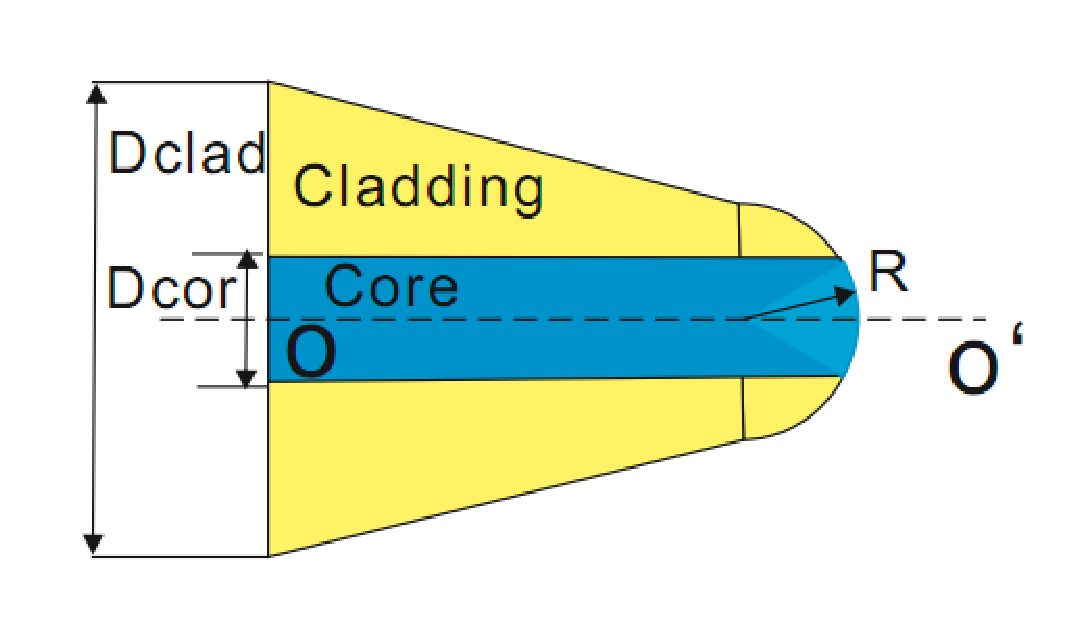
\includegraphics[width=0.4\textwidth]{bilder/lense_fiber_01}
\label{fig:lense_fiber_01}
}
\hfill
\subfigure[Tapered core TLF.]{
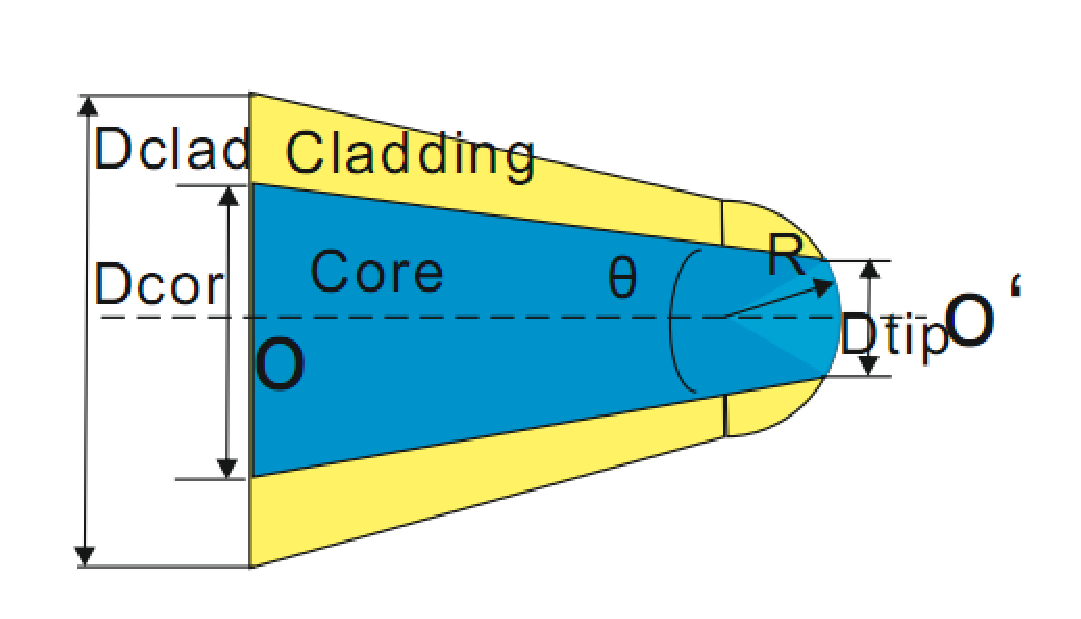
\includegraphics[width=0.4\textwidth]{bilder/lense_fiber_02}
\label{fig:lense_fiber_02}
}
\label{fig:two_TLF}
\caption{Two types of Tapered and Lensed Fibers}
\end{figure}

The Tapered Cladding TLF Fig.\ref{fig:lense_fiber_01} shows that its cladding diameter decreases along the axis and its core diameter is a constant. For the Tapered Core TLF Fig.\ref{fig:lense_fiber_02} its cladding diameter and core diameter both decrease along the axis. \cite{TLF_mode_transforming} develops method to estimate the performance of both type of TLF.  And results show that the performance of the first type of TLF agrees well with the estimation and that of the second type is unpredictable. 

Create two TLF models from each type and test the performances in CST MWS. The following Tab.\ref{tab:model_fiber_configuration} indicates the corresponding configurations.

\begin{table}
\begin{tabular}{ccc}
\hline
							&Tapered Cladding&Tapered Core\\
\hline
$R(\mu m)$ & $6$						 &$6$	\\
refractive indices(core)&$1.68$&$1.66$\\
refractive indices(cladding)&$1.68$&$1.66$\\
$D_{clad}(\mu m)$ &	$17$ &	$17$\\
$D_{core}(\mu m)$ & $10$ &	$17$\\
$D_{tip}(\mu m)$  & --   &	$10$\\
\hline
\end{tabular}
\caption{The Configurations of the TLF Models}
\label{tab:model_fiber_configuration}
\end{table}



\begin{figure}
\setlength{\abovecaptionskip}{0pt}% 
\flushleft
	\subfigure[sub1]{
	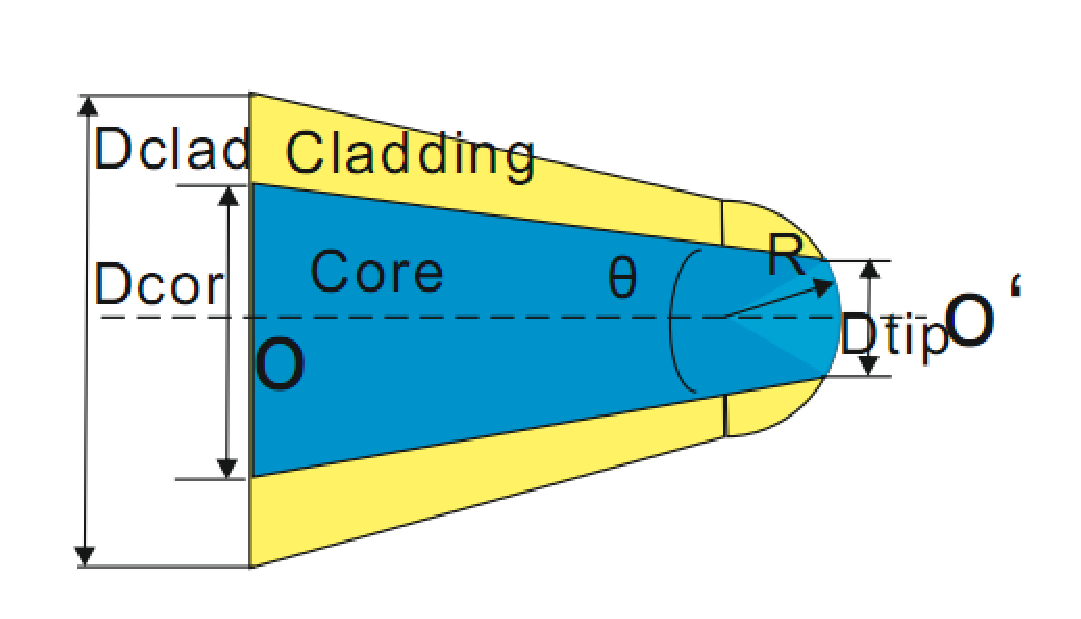
\includegraphics[width=0.23 \textwidth]{bilder/lense_fiber_02}
	\label{fig:subfigure1}%
	}

 	\subfigure[sub2]{
 	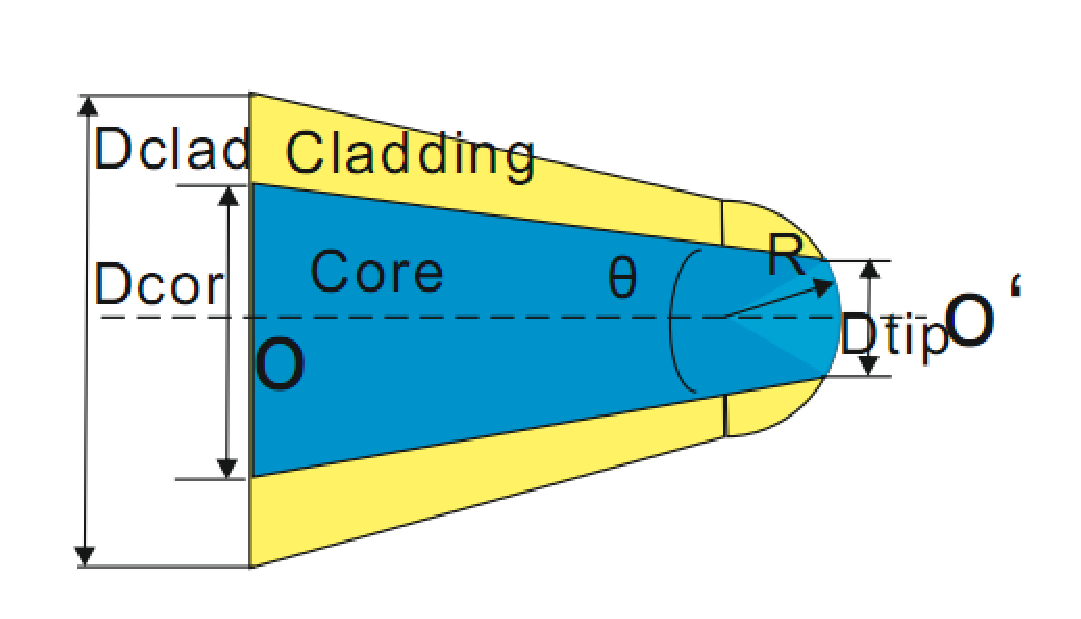
\includegraphics[width=0.23 \textwidth]{bilder/lense_fiber_02}
 	\label{fig:subfigure2}
 	}
 	 	\subfigure[sub2]{
 	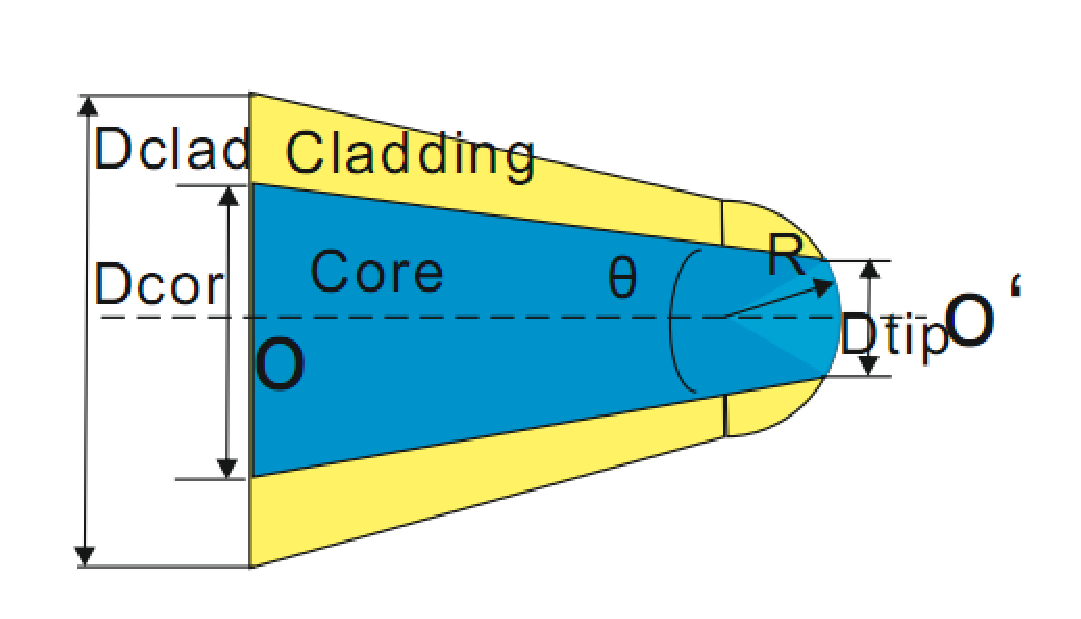
\includegraphics[width=0.23 \textwidth]{bilder/lense_fiber_02}
 	\label{fig:subfigure3}
 	}
 	 	\subfigure[sub2]{
 	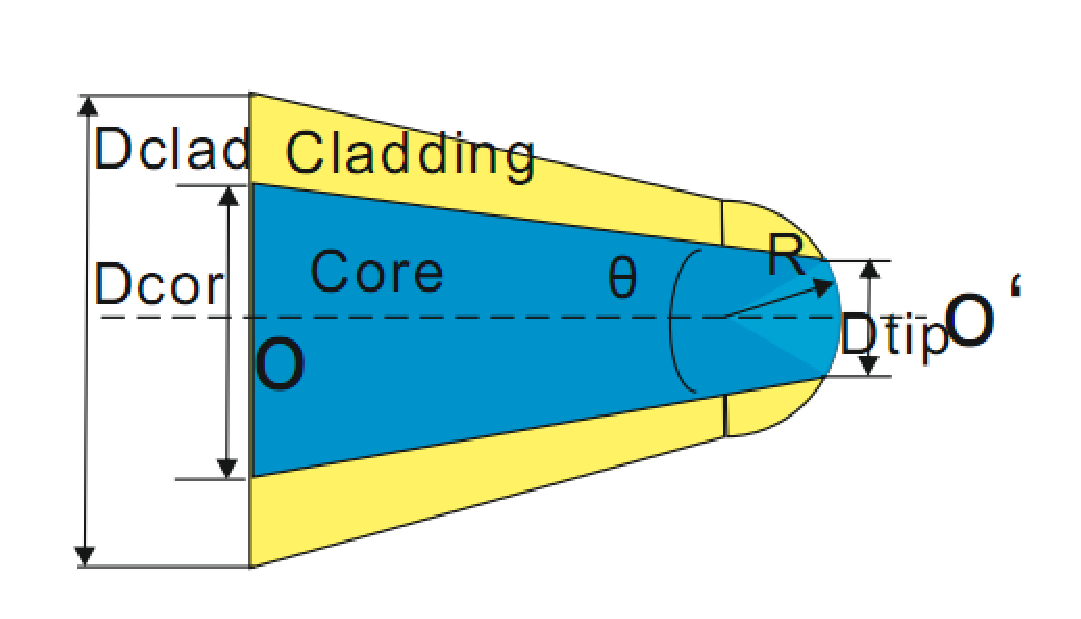
\includegraphics[width=0.23 \textwidth]{bilder/lense_fiber_02}
 	\label{fig:subfigure4}
 	}
 	 	\subfigure[sub2]{
 	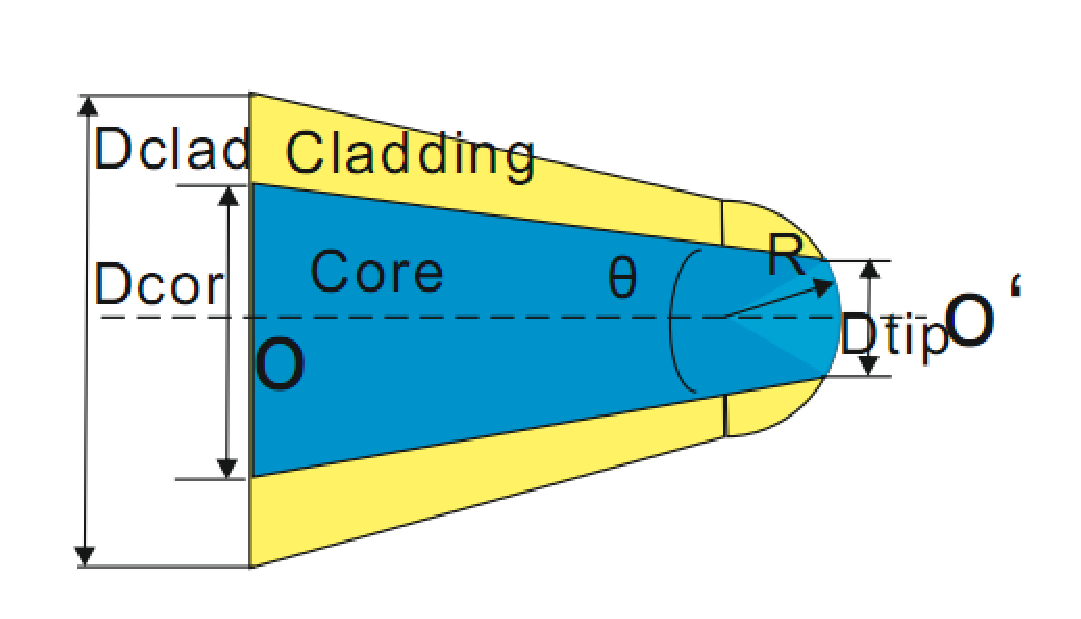
\includegraphics[width=0.23 \textwidth]{bilder/lense_fiber_02}
 	\label{fig:subfigure5}
 	}
\end{figure}

%2.20
The fowllowing is the E-Field demonstration in the xz-plane.
\begin{figure}
	\subfigure[E-Field demonstration of Tapered cladding TLF]{
		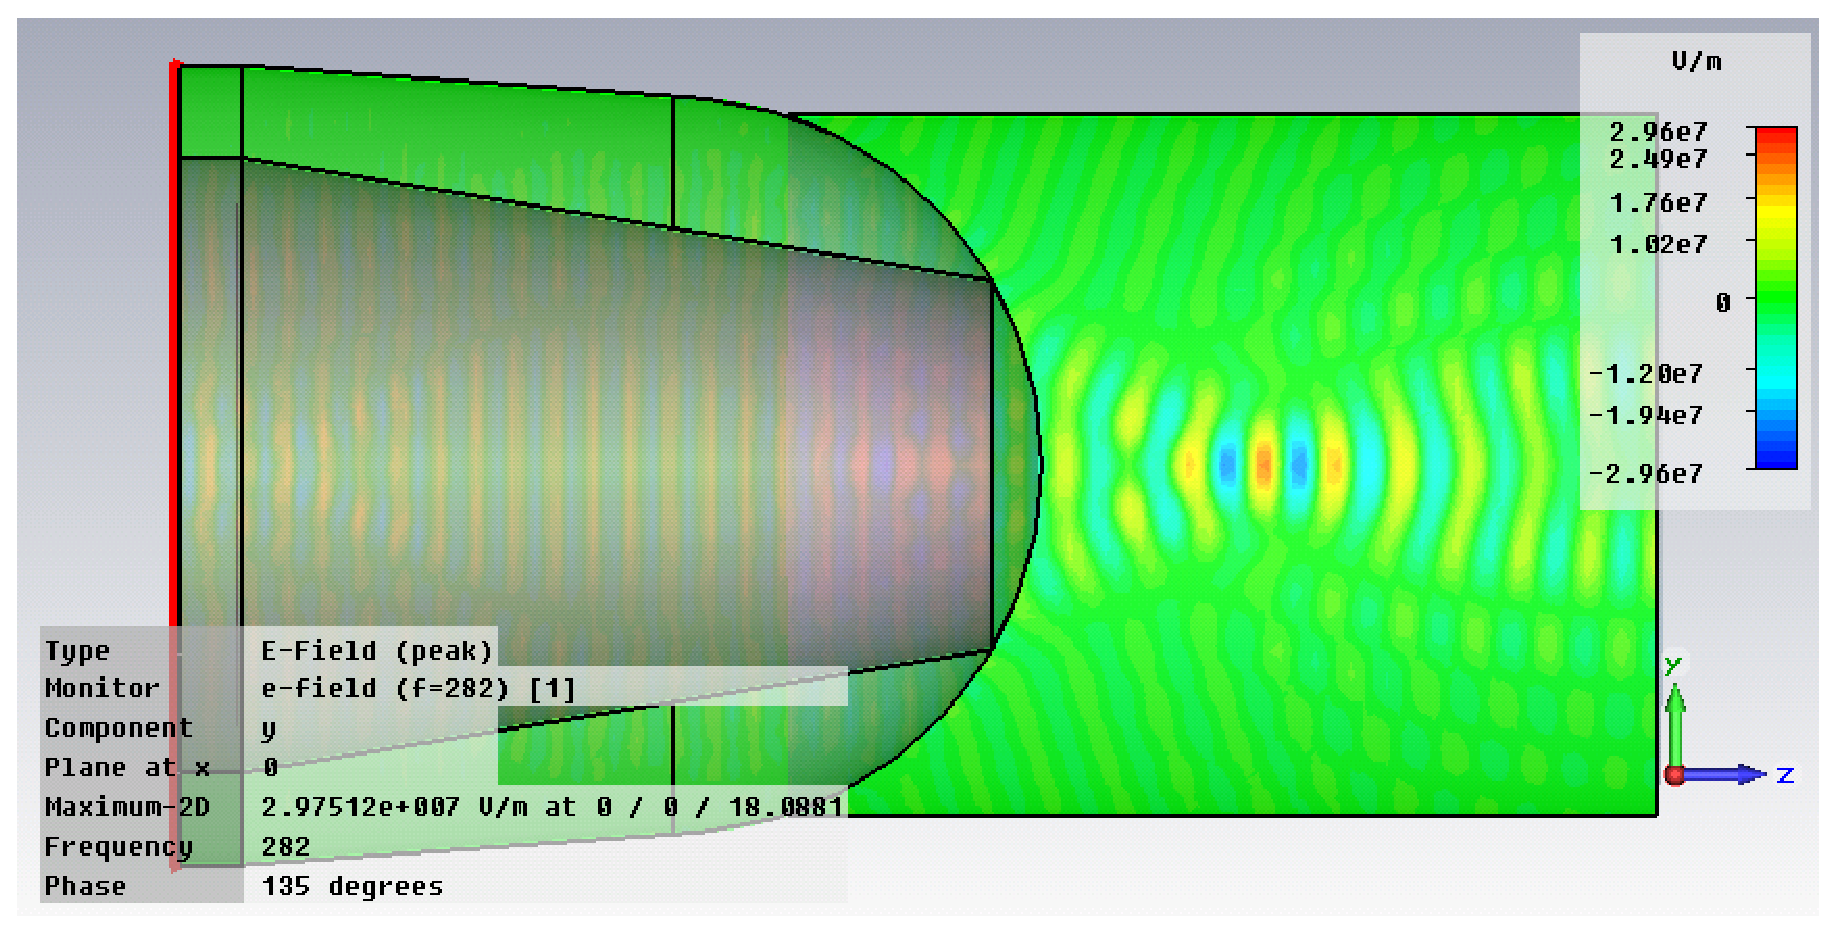
\includegraphics[width=0.4 \textwidth]{bilder/cst_lensed_fiber_efield}
 		\label{fig:Tapered_cladding_efield}
	}
	\subfigure[E-Field demonstration of Tapered core TLF]{
		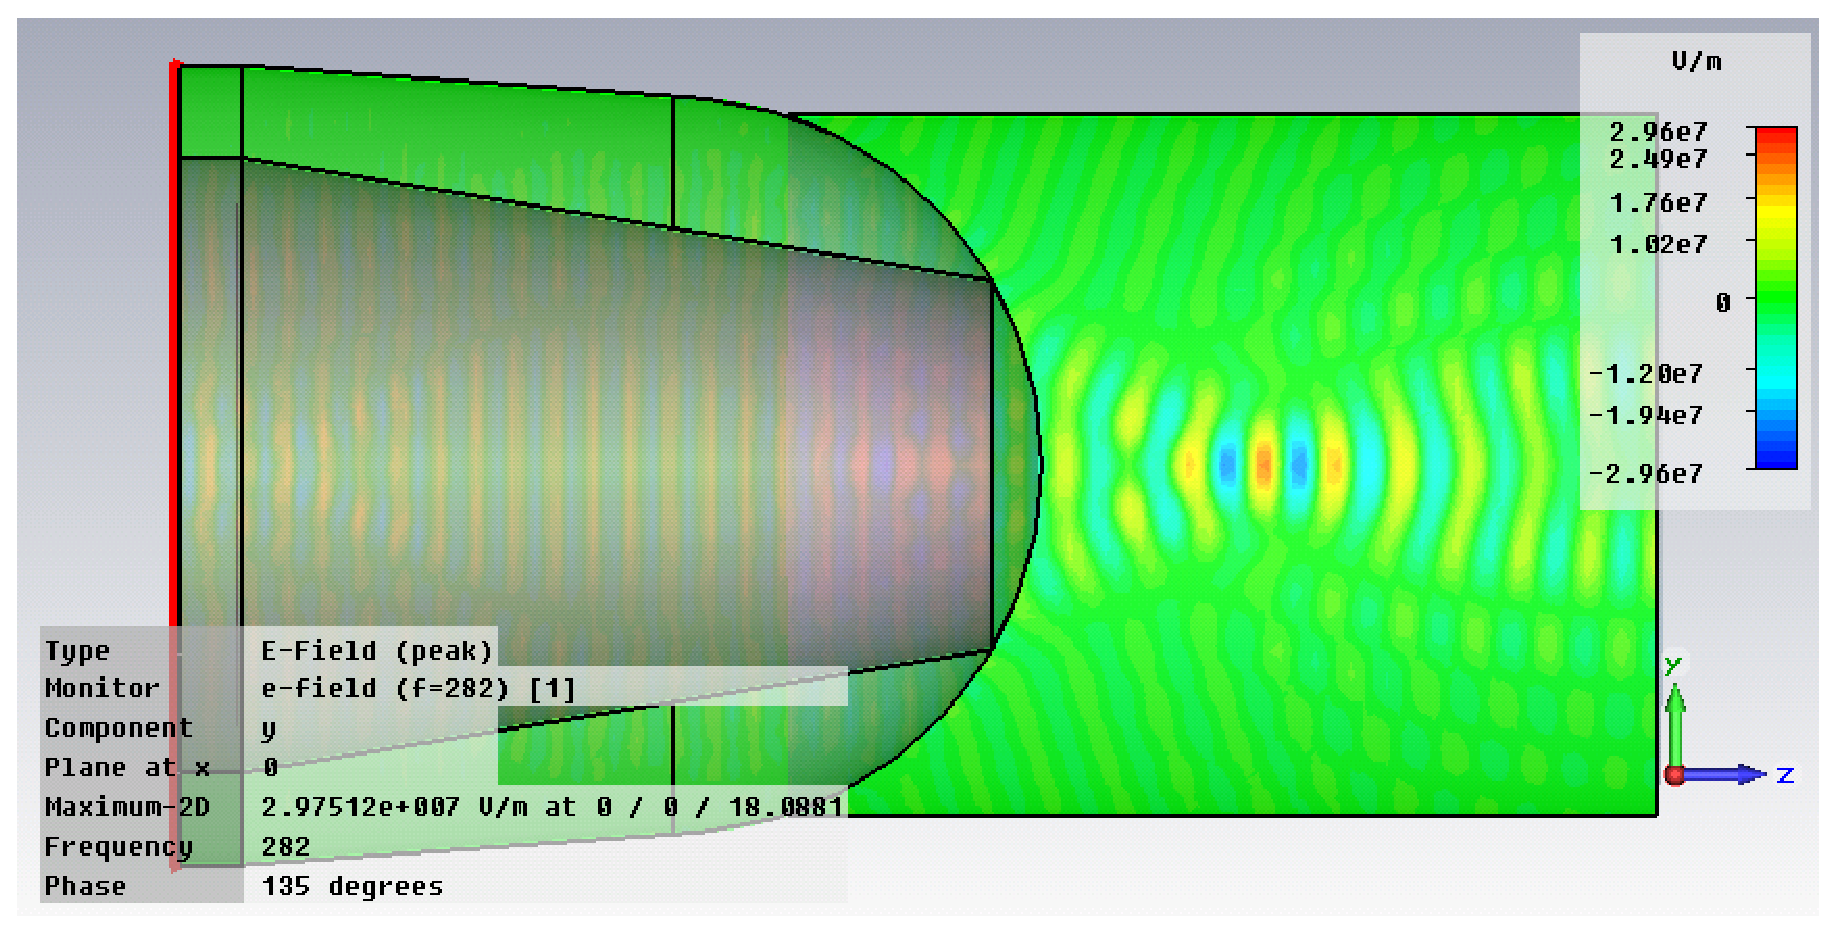
\includegraphics[width=0.4 \textwidth]{bilder/cst_lensed_fiber_efield}
 		\label{fig:Tapered_core_efield}	
	}
	\caption{E Field demonstration}
\end{figure}
As is in section lense theory introduced, the minimum spot located not exactly at the focal length. By using the location of PP and that of MP the MS can be estimated. The theoretical distance from lens end to PP is $xx \mu m$ and the distance from lens end to MP is  $xx \mu m$. Backword $3/4$ LAM form PP, the MS is founded at about $xx \mu m$far from lens end. Through The following figure is the theoretical beam propagation of the lense model.
Load the its beam propagation detail into \textbf{Matlab} workspace and check the beam power distribution in different distance. Fig.(\ref{}-\ref{}).%2D and 3D

\begin{figure}
\end{figure}
 
Draw Fig.\ref{}-\ref{} to illustrate the beam Spot size diameter along the longitude axis.

\begin{figure}
\caption{Curve of Spot size diameter}
\end{figure}
From Fig.\ref{tapered cladding} that the minimum spot size locate at $xxx \mu m$ from lense end and spot size equal about $1.7 \mu m$. While in Fig.\ref{tapered core} that the minimum spot size is found at  $xxx \mu m$ from lense end and spot size equal about $1.5 \mu m$. Thus it is concluded that tapered core TLF has a bit higher focal performance. By rechecking the properties in Tab.\ref{} both TLF model are acceptable for the following development. In this article the Tapered core TLF will be used for further simulations. 

\subsection{Modelling the Fiber to Chip}
\label{sect:model_model_fiber2chip}
%fiber2chip_modelings
As beginning of this chapter the waveguide model will be approximate with a rectangle waveguide. Place the waveguide at the working distance $4\mu$m before the TLF.  Fig.\quad\ref{fig:coupling_e_field} from the simulation of this configuration shows the E-Field spread more widely at the interface of the waveguide than that in the case without blockage of the waveguide and apparently a great part of E-Field infiltrate into the waveguide rather than accepted by guide. Thus by checking the S-parameter of this simulation Fig.\ref{fig:orignial_coupling_efficiency},which present the S21 in frequencies, the coupling efficiency ($S_{21}$) is about $48.8\%$ at the working frequency $282$HZ($\lambda=1064$nm). This result will act as the reference sample for the other simulations. 
\begin{figure}[!ht]
\centering
	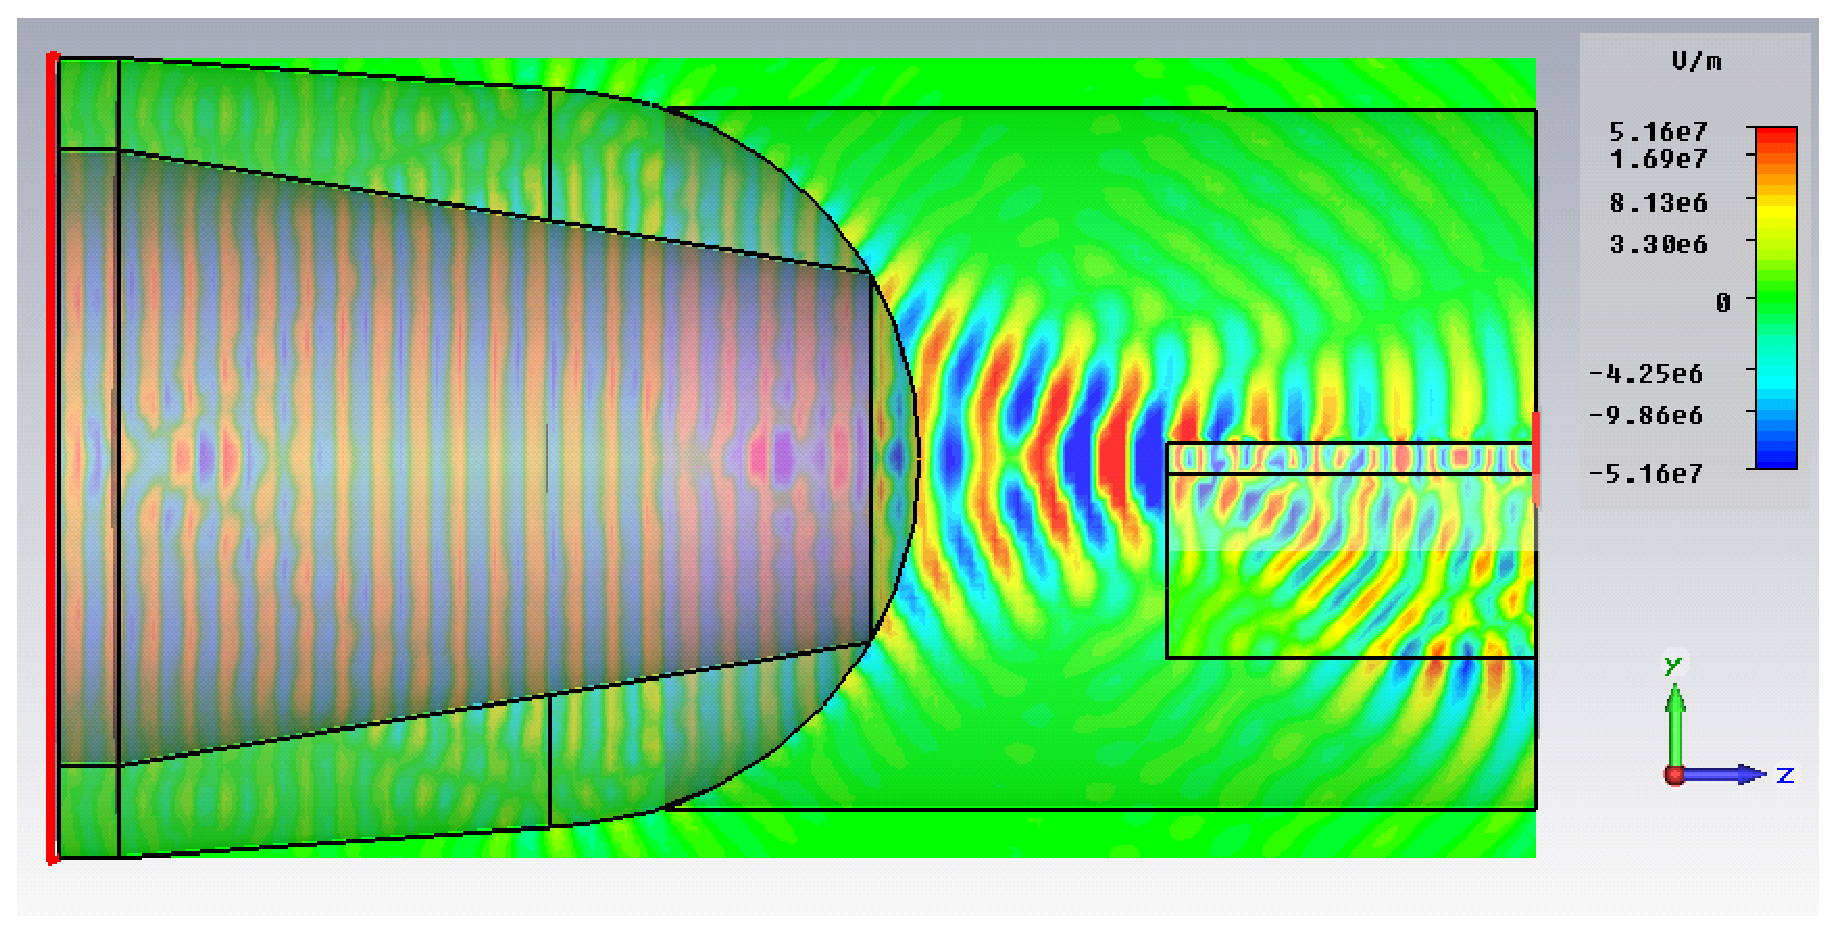
\includegraphics[width=0.7 \textwidth]{bilder/cst_basic_waveguide_efield}
	\label{fig:coupling_e_field}
	\caption{E-Field demonstration by coupling.}
\end{figure}
Furthermore people can analyze the power distribution at the guide from Fig.\quad\ref{fig:power_distribution}( see Appendix.\quad\ref{app:powwer_distribution} ). In the figure it can be found that about $40\%$ power propagates in the guide while another $40\%$ in the substrate and the rest is losing in the air or reflecting.
\begin{figure}
\centering
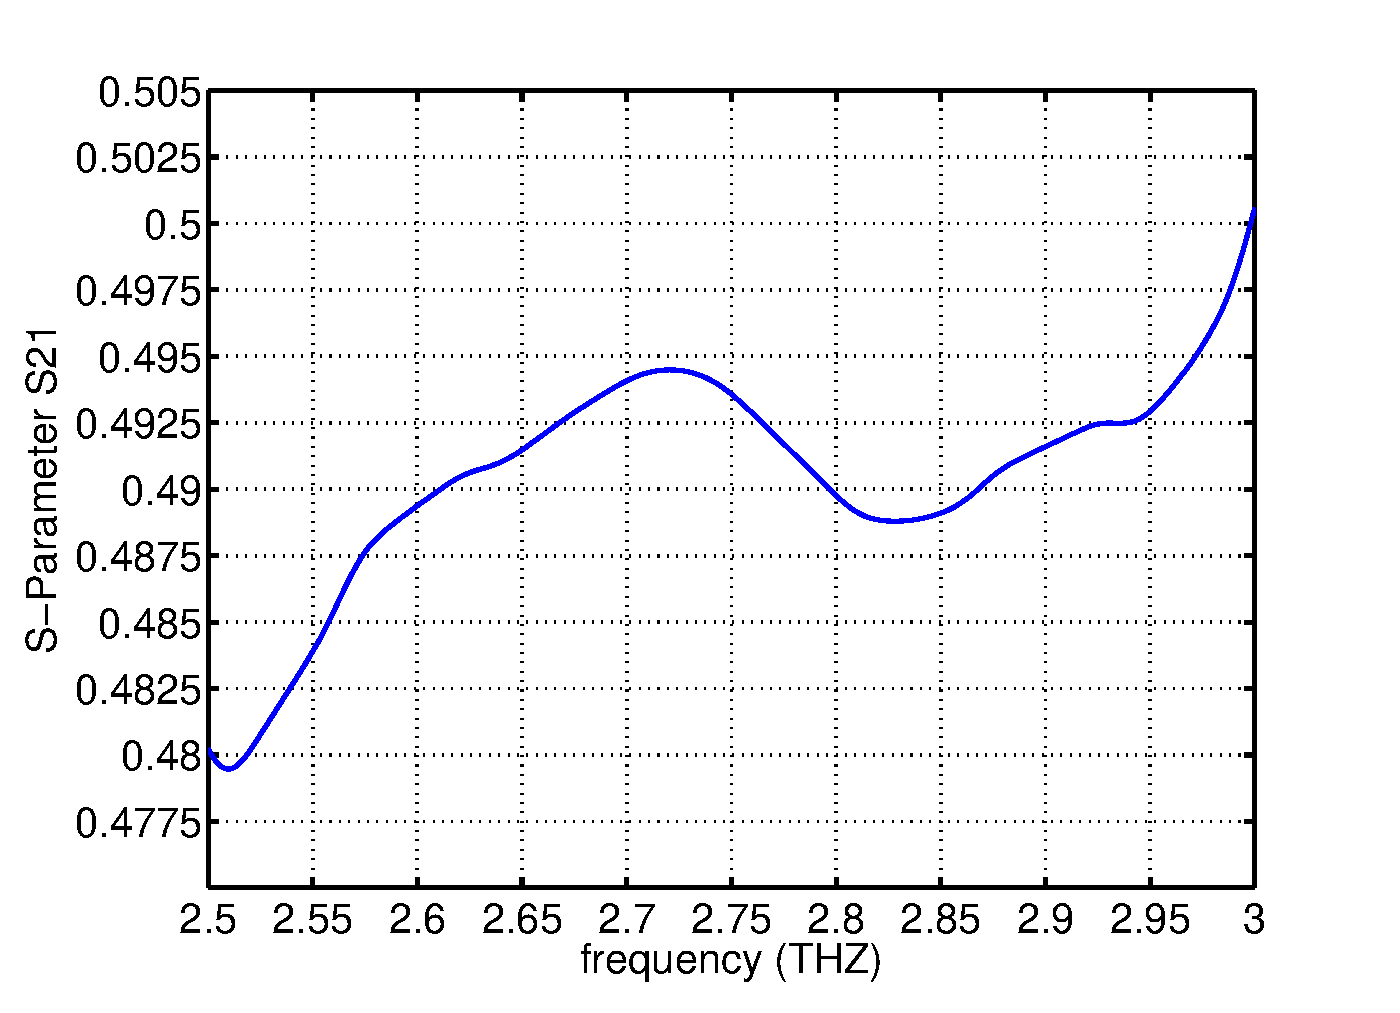
\includegraphics[width=0.7\textwidth]{bilder/original_coupling_efficiency}
\caption{coupling efficiency in Frequency area.}
\label{fig:orignial_coupling_efficiency}
\end{figure}
\begin{figure}[!ht]
\centering
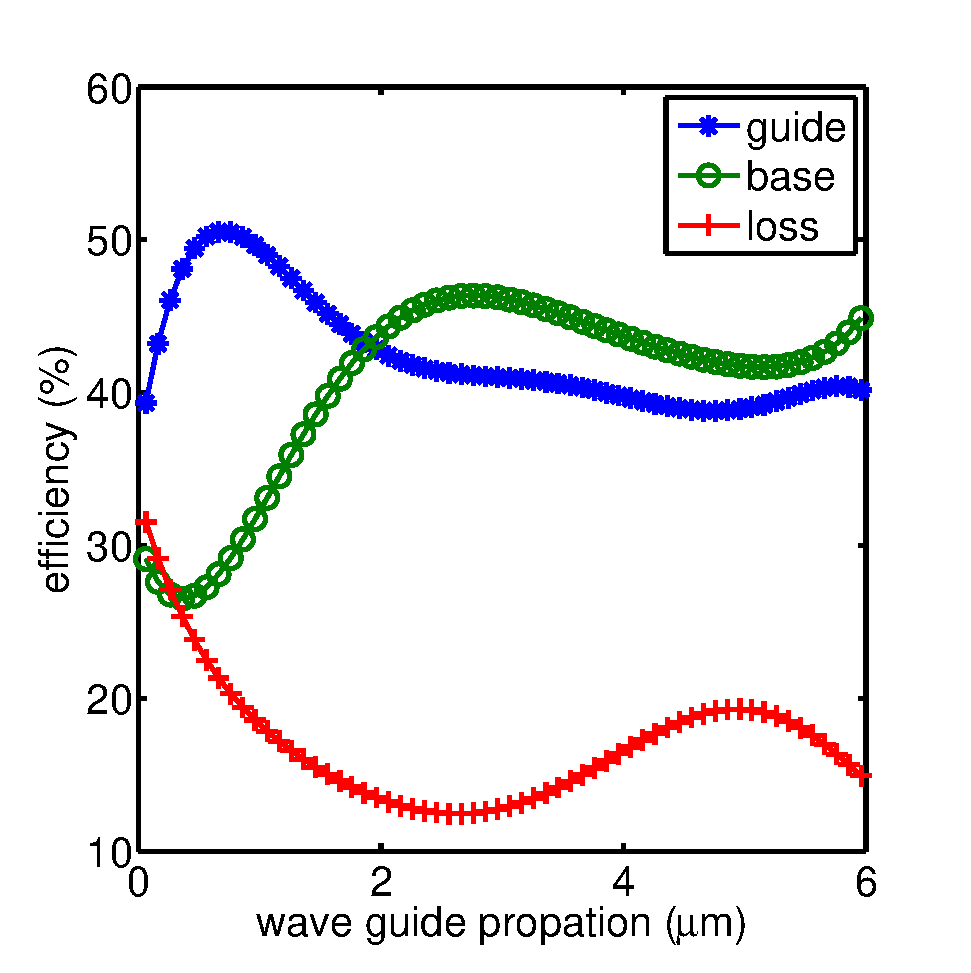
\includegraphics[width=0.7\textwidth]{bilder/power_distribution}
\caption{power distribution along the waveguide.}
\label{fig:power_distribution}
\end{figure}


%
\chapter{Optimize}
\label{chp:optim}
%optimize_introduction
This chapter aims to discuss the optimization methods to improve the Fiber-to-Chip coupling efficiency. Five proposals will be obtained in this chapter. One is to relocate the waveguide. Another is to replace the round condition of the simulation setup with oil. In the third proposal we will consider to change the composed material of the waveguide.  The application of a taper interface at the beginning of the waveguide is involved in the next consideration. At last we are going to mount a lens at the waveguide end face.


\section{Coupling by location shifting}
\label{sect:optim_shift}
%\section{Coupling by location shifting}
%coupling_shifting
As a 3D model the waveguide can be shifted on transverse (Fig. \ref{fig:shift_x_axis} and Fig. \ref{fig:shift_y_axis}) or longitude (Fig. \ref{fig:shift_z_axis}) directions.
\begin{itemize}
\item Shift the waveguide along X-Axis: Relocate the waveguide from $-0.5\mu$m to $0.5\mu$m:
\begin{figure}[!ht]
\centering
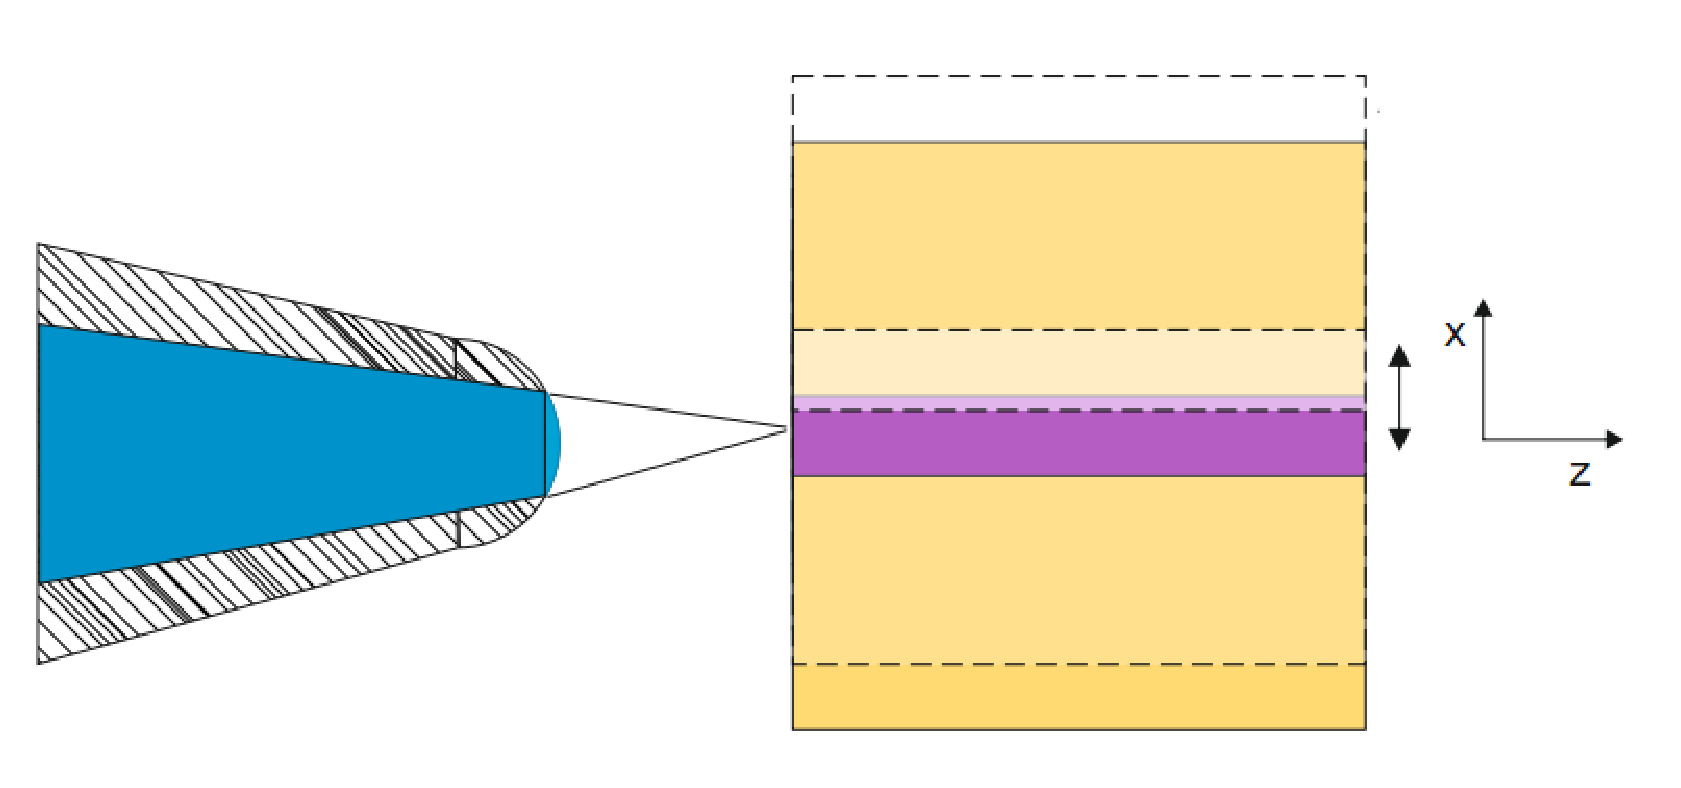
\includegraphics[width=0.7\textwidth]{bilder/shift_x_axis}
\caption{Displacing the waveguide along x-axis}
\label{fig:shift_x_axis}
\end{figure}
\item Shift the waveguide along Y-Axis: Relocate the waveguide from $-0.5\mu$m to $0.5\mu$m:
\begin{figure}[!ht]
\centering
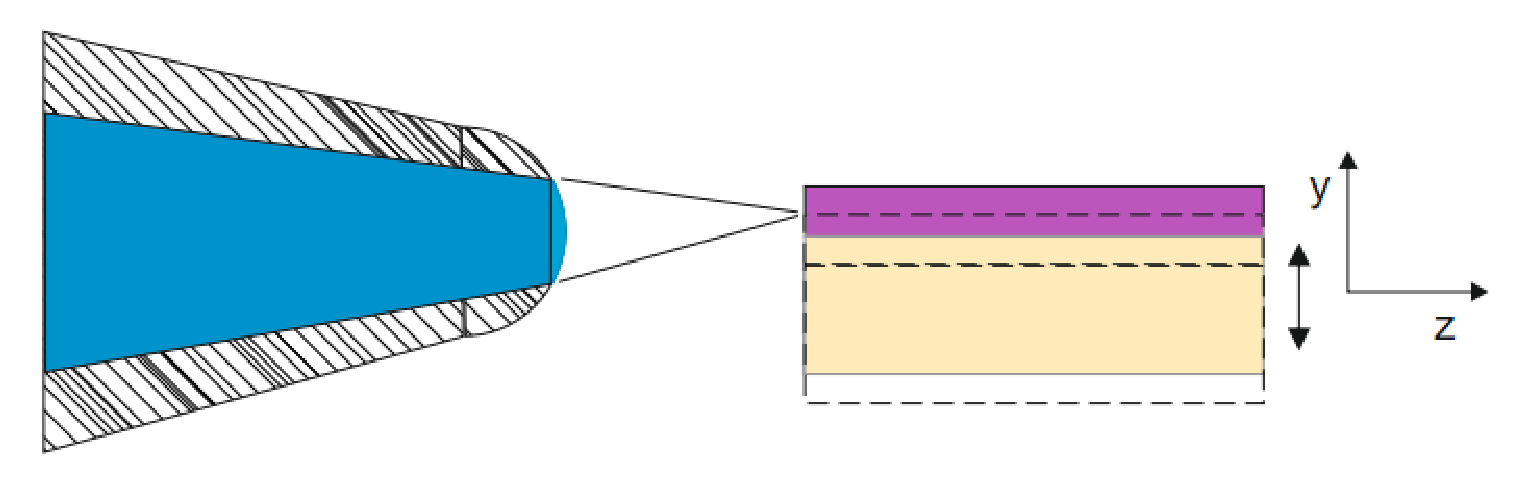
\includegraphics[width=0.7\textwidth]{bilder/shift_y_axis}
\caption{Displacing the waveguide along y-axis}
\label{fig:shift_y_axis}
\end{figure}
\item Shift the waveguide along Z-Axis: Relocate the waveguide from $-0.5\mu$m to $0.5\mu$m:
\begin{figure}[!ht]
\centering
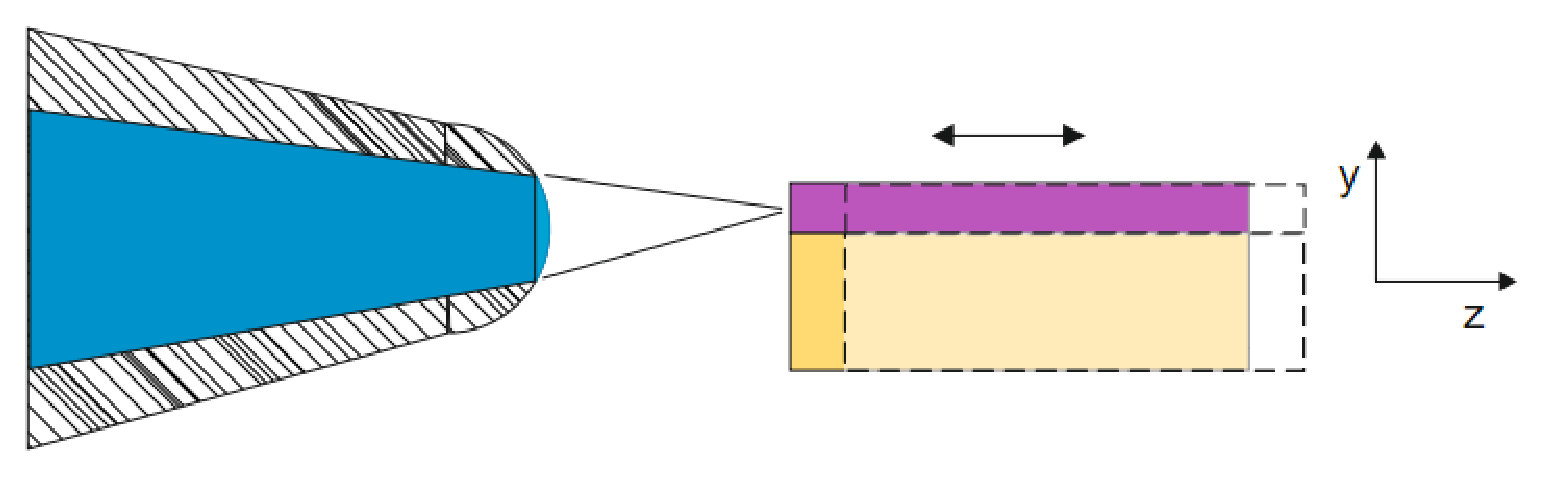
\includegraphics[width=0.7\textwidth]{bilder/shift_z_axis}
\caption{Displacing the waveguide along z-axis}
\label{fig:shift_z_axis}
\end{figure}
\end{itemize}

Performe above arrengments and record their simulation results $|S_{21}|$ in Tab. \ref{tab:shift_result}:
\begin{table}
\caption{Coupling efficiency by shifting the waveguide along X,Y and Z-Axis}
\centering
\begin{tabular}{c|ccc}
\hline
Shift distance & X-Asis & Y-Axis & Z-Axis \\
\hline
$-0.5\mu$m 		&$32.4\%$	&$32.4\%$&$46.6\%$	\\
$-0.4\mu$m		&$37.3\%$	&$36.5\%$&$47\%$	\\
$-0.3\mu$m 		&$41.9\%$	&$41.3\%$&$48.2\%$	\\
$-0.2\mu$m	  &$45.5\%$	&$45.2\%$&$49.1\%$	\\
$-0.1\mu$m		&$48\%$	&$47.8\%$&$49.1\%$	\\
$0\mu$m			  &$48.9\%$	&$48.9\%$&$48.9\%$	\\
$0.1\mu$m			&$47.8\%$	&$48.4\%$&$48.9\%$	\\
$0.2\mu$m			&$45.5\%$	&$46.4\%$&$49.4\%$	\\
$0.3\mu$m			&$41.9\%$	&$42.9\%$&$49.7\%$	\\
$0.4\mu$m			&$37.5\%$	&$38.5\%$&$49.5\%$	\\
$0.5\mu$m			&$32.3\%$	&$33.1\%$&$48.8\%$	\\
\hline
\end{tabular}
\label{tab:shift_result}
\end{table}
According these results we can draw their curves in Fig. \ref{fig:shift_curve}, which presents us their coupling efficiency behavior. It is obvious that the coupling efficiency falls very quickly for vertical or horizontal shifting, while it stays relative stable for longitude displacement. From this Figure we can also reveal that coupling efficiencies are symmetric due to positive and negative X-Axis shifting. While the coupling efficiencies due to negative and positive Y-Axis shifting are not symmetric. This trend can be explained by the geometric characters of the waveguide, which is same in X-Dimension and different in Y-Dimension. And the highest coupling efficiency due to shifting along Z-Axis stands not at working distance $4\mu$m but $4.3\mu$m, which agree with the estimation of minimum spot location about $4.26\mu$m at section \ref{sect:model_model_model_TLF}. Alought the minimum spot location lies not on the working distance $4\mu$m, displacement of the waveguide can not obviously improve the coupling efficiency. Hereby the working distance will be maintained in following simulations.
  
\begin{figure}[!ht]
\centering
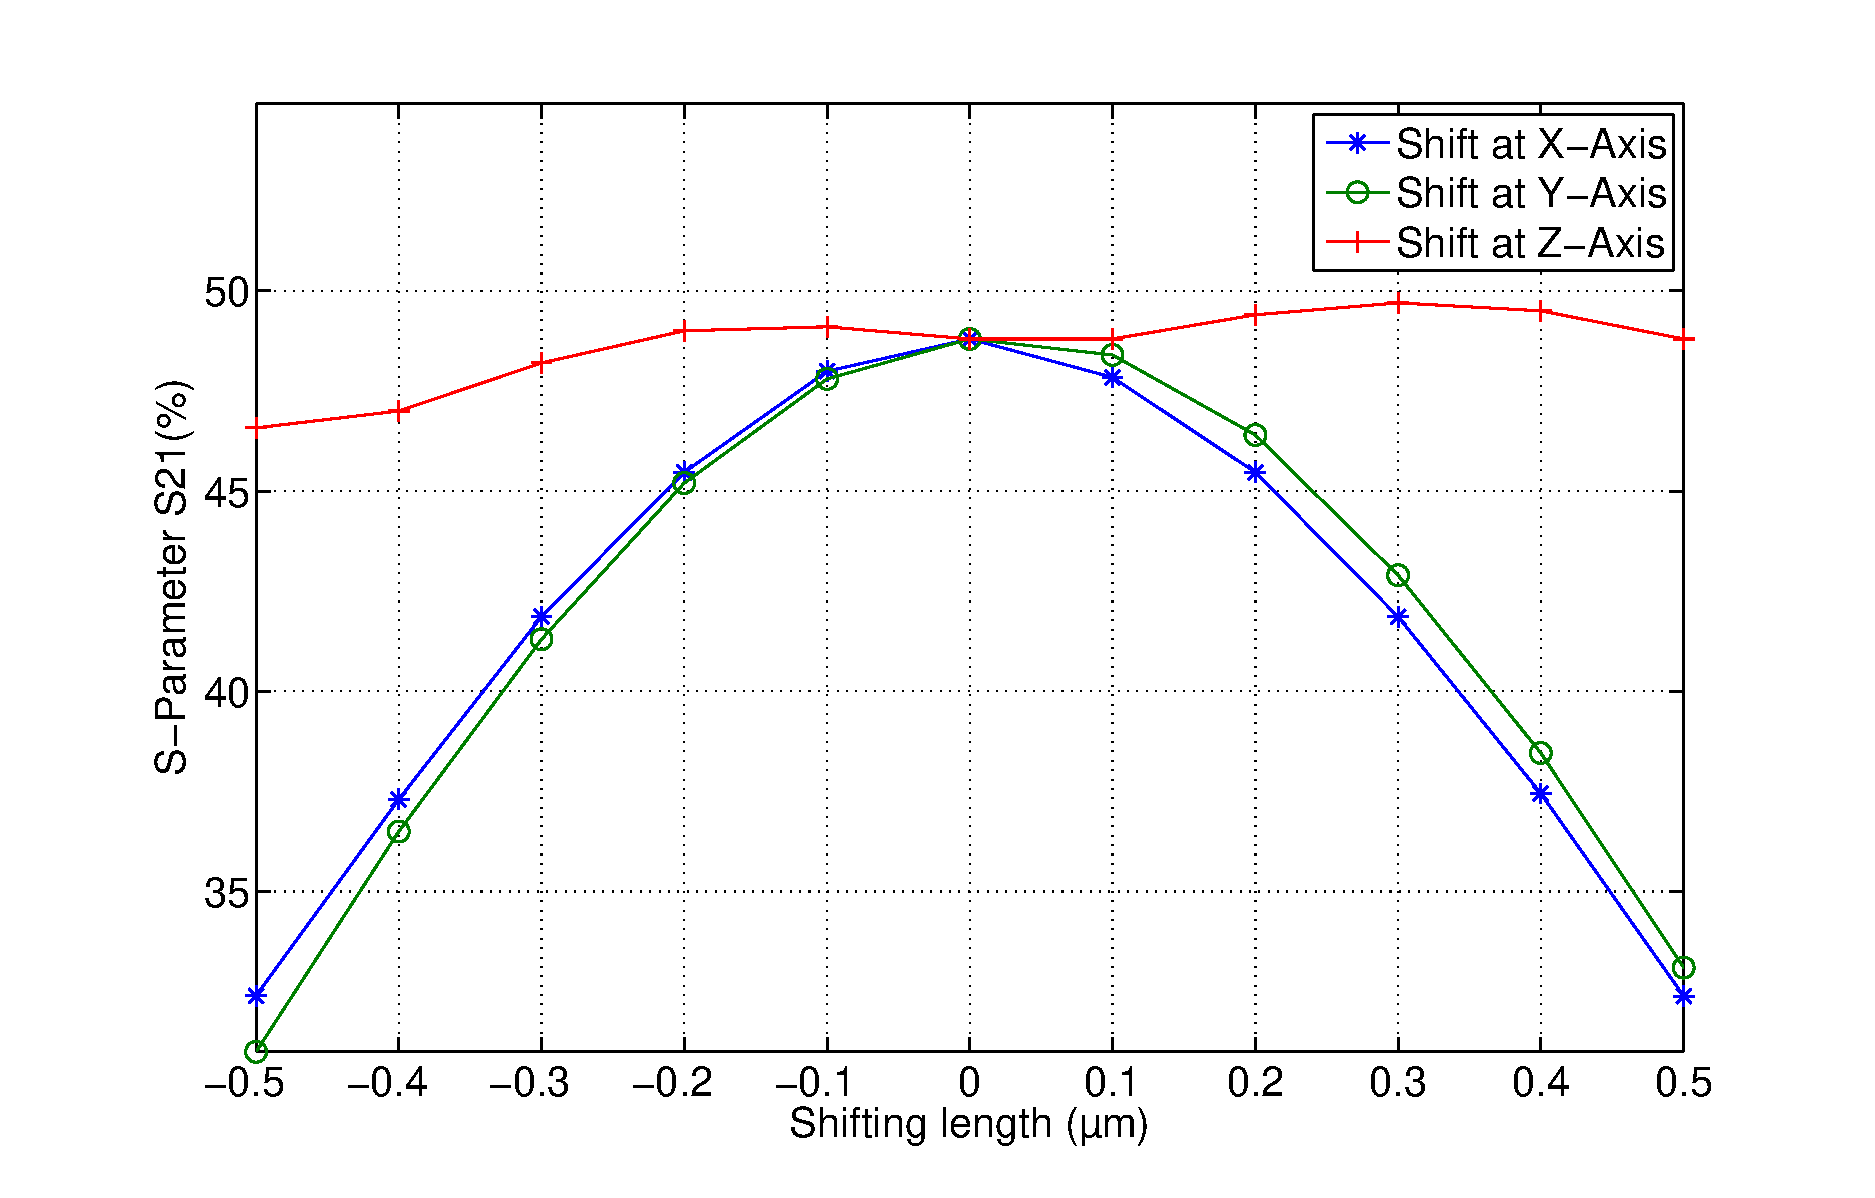
\includegraphics[width=0.8\textwidth]{bilder/shift_curve}
\caption{Coupling efficiency due to the displacement of the wavguide.}
\label{fig:shift_curve}
\end{figure}


\section{Simulation in oil environment}
% coupling_oil
In this section a different background environment is contained in the coupling simulation. For the practical experiment there are no many options for changing the environment. Here the coupling configuration in section \ref{sect:model_model_fiber2chip} will be placed in an environment full of oil. Changing the background may greatly affect the working distance of the  TLF. Therefore determining the new working distance is necessary before couple the TLF to the waveguide.  Similar as in section \ref{sect:model_model_model_TLF} the spot size curve Fig. \ref{fig:oil_spot_curve} can be drawn by loading data from the simulation of TLF beam propagation in oil. Here we can tell from the spot size cure that the minimum spot in oil lies at the position more remote than the original minimum spot in air.    
\begin{figure}[!ht]
\centering
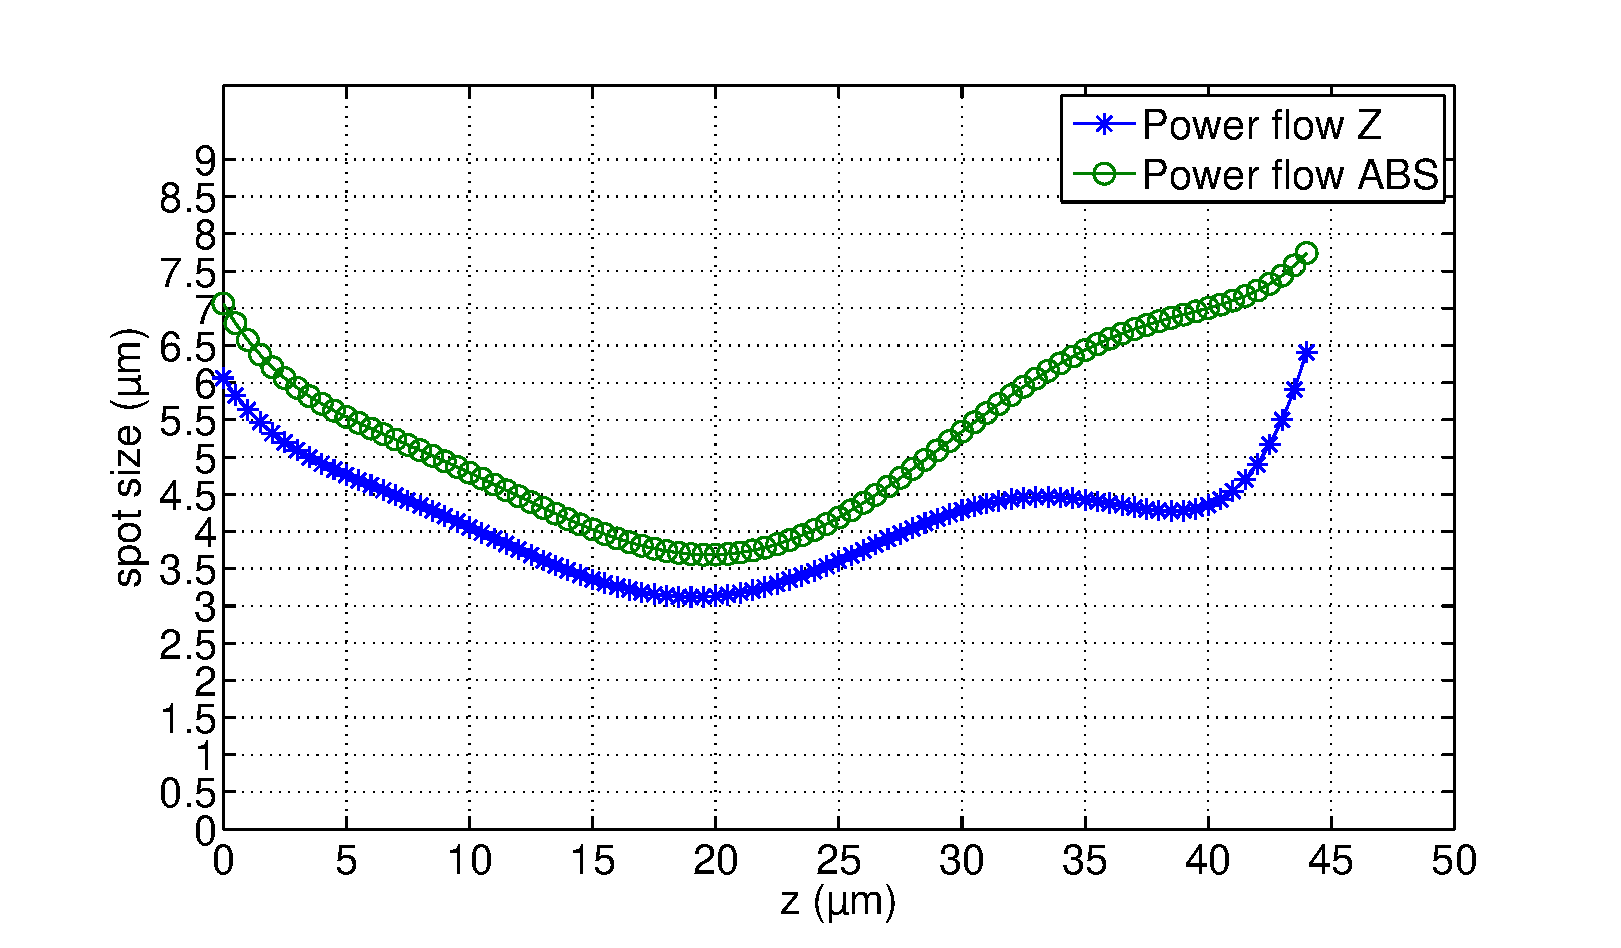
\includegraphics[width=0.7\textwidth]{bilder/spot_curve_oil}
\caption{Spot size curve of TLF in oil.}
\label{fig:oil_spot_curve}
\end{figure}
Place the waveguide at the new working distance and execute the coupling simulation. The coupling efficiency of Fiber-to-Chip in oil can be found in curve Fig. \ref{fig:oil_coupling_curve}. The result shows that the coupling efficiency at working frequency $282$THZ achieves about $34.5\%$, which is lower than that of the original configuration in section \ref{sect:model_model_model_TLF}.
\begin{figure}[!ht]
\centering
\includegraphics[width=0.7\textwidth]{bilder/s21_oil_curve}
\caption{Coupling efficiency between TLF and the rib waveguide due to frequency domain in oil background.}
\label{fig:oil_coupling_curve}
\end{figure}


\section{Different refract indexes}
%\section{Different refract index}
It is obvious that the refractive index of the waveguide affects the coupling ability. In this section the effect of varying refractive index for coupling will be discussed. 
We will keep the substrate setup and test the guide in refractive indexes form $1.6$ to $2.5$ in this section.\\

\begin{figure}[!ht]
\centering
\includegraphics[width=0.7\textwidth]{bilder/s21_refractive_index}
\caption{Coupling efficiency between TLF and the rib waveguide due to refractive index.}
\label{fig:refractive_index}
\end{figure}

Simulation results are mapped into Fig. \ref{fig:refractive_index}. It can be told from the figure that the coupling ability rise sharply within $n=1.6$ to $1.8$ then decline softly due to the increasing of refractive indexes. The highest value of the coupling efficiency among the arrangements in this section is about $62.6\%$ when the guide is composed of material of $n=1.8$.\\
Surely, it is not possible to find the material of any refractive index. If we want to improve the coupling ability by this means, we can only choose a material with a refractive index close to $n=1.8$.


\section{Tapered waveguide}
%\section{Tapered waveguide}
%tapered_waveguide
Tapered waveguide is inhomogeneous waveguide on shape, whose dimensions in the tapered section changes slowly along the longitude dirccetion\cite{linear_tapered_waveguides}. Tapered structure enables the waveguide to receive more light so that improve the coupling efficiency between beam source and waveguide.  
The author of \cite{design_fabrication_tapered_waveguide} has presented two general types of tapered waveguide: conventional taper like top view Fig. \ref{fig:conventional_taper} and inverse taper like top view  Fig. \ref{fig:inverse_taper}. For a conventional taper the entry is wider than the exit while for an inverse taper the entry is narrower than the exit. In this section the conventional taper will be discussed.
\begin{figure}[!ht]
\centering
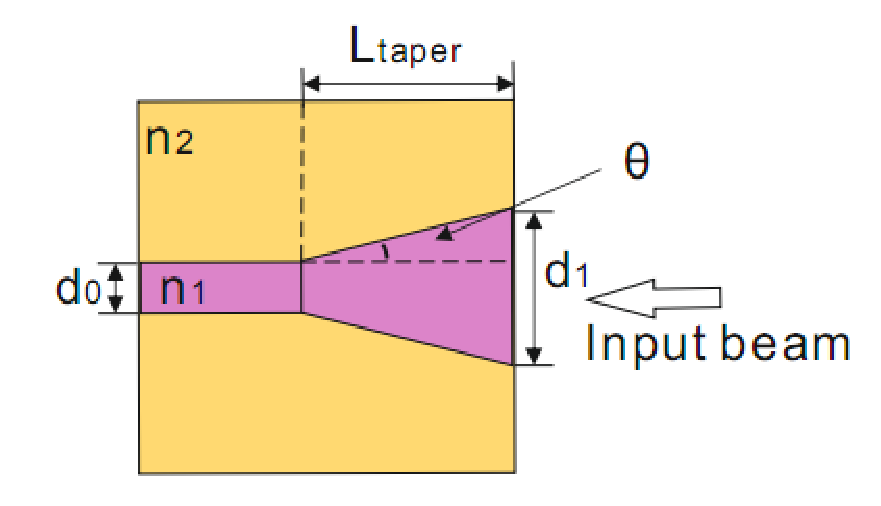
\includegraphics[width=0.7\textwidth]{bilder/convernational_taper}
\caption{Schema of a conventional taper.}
\label{fig:conventional_taper}
\end{figure}
\begin{figure}[!ht]
\centering
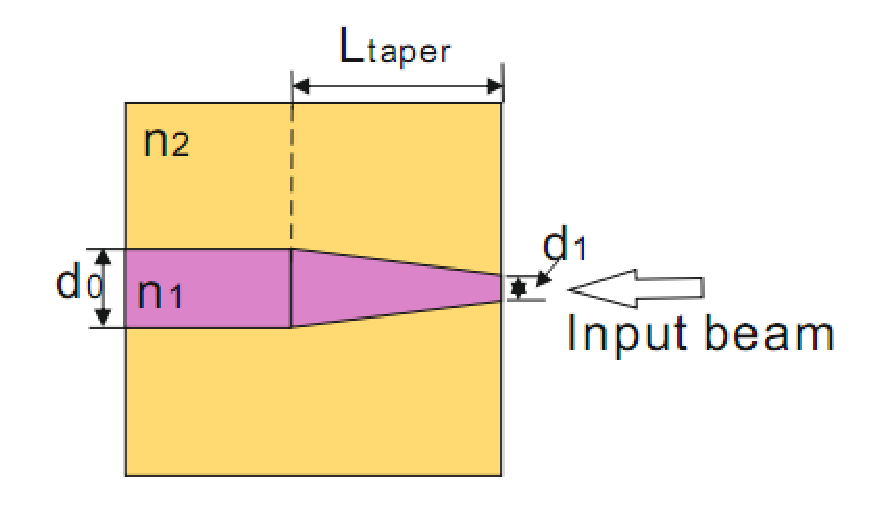
\includegraphics[width=0.7\textwidth]{bilder/inverse_taper}
\caption{Schema of a inverse taper.}
\label{fig:inverse_taper}
\end{figure}

Two properties, the width $d_{1}$ of a taper interface and the divergence angle $\theta$ of the taper, of the taper may strongly affect the coupling efficiency. For convenient calculations our simulations will be arranged respectively due to variations of taper width and taper length $L_{taper}$ instead of divergence angle.


\subsection{Tapered waveguide due to interface width} 
%\subsection{Tapered waveguide due to interface width} 
%tapered_width
The taper width affects the acceptable scale of the waveguide. The beam spot diameter at the working distance is about $1.5\mu$m, while the regular waveguide has smaller dimensions (w=$1\mu$m and h=$0.5\mu$m). In order to catch a complete view we discuss the tapered width starting with $1.2\mu$m to match the beam spot. Fig. \ref{fig:tapered_waveguide_wxx} presents the coupling behavior of the tapered waveguide along the variation of the interface width. From the figure it can be told that the coupling efficiency of this arrangement rise firstly with the width increasing and achieve its peak value at the width $d_{1}=2\mu$m and $2.2\mu$m. Then the efficiency falls as the interface width increasing. This tendency can be explained that a wider interface can confine more incident rays into the propagation tunnel but if the interface expands continually, other aspects, such as the divergence angle, may cause the decline of the coupling ability over the effect of the interface width.\\ 

\begin{figure}[!ht]
\centering
\includegraphics[width=0.7\textwidth]{bilder/tapered_waveguide_wxx}
\caption{Coupling efficiency between TLF and tapered waveguide with constant taper length $= 5.5\mu$m due to the variations of the interface width.}
\label{fig:tapered_waveguide_wxx}
\end{figure}


\subsection{Tapered waveguide due to taper length}
%\subsection{Tapered waveguide due to taper length}
%tapered_length
The value of the divergence angle is also a important character of the tapered waveguide to determine the coupling ability. The author of \cite{study_linear_tapered_waveguides} has presented that the smaller the divergence angle is, the more power of fundamental mode propagates in the taper. In order to simplify the modeling process the variation of taper length will be performed in the following coupling simulations to discuss the effect of the divergence angle.
We will keep the taper interface width of the waveguide as a constant of $2\mu$m and change the taper length from $2\mu$m to $5.5\mu$m in following simulations.\\
  
\begin{figure}[!ht]
\centering
\includegraphics[width=0.7\textwidth]{bilder/tapered_waveguide_dxx}
\caption{Coupling efficiency between TLF and tapered waveguide due to taper length and taper width $= 2\mu$m}
\label{fig:tapered_waveguide_dxx}
\end{figure}
The coupling behavior of the arrangement, the taper length vary from $2\mu$m to $5.5\mu$m, is shown in Fig. \ref{fig:tapered_waveguide_dxx}.  The figure illustrate that the coupling efficiency increase monotonously with the taper length expanding. After taper length $4.5\mu$m of the coupling efficiency rise more and more gently, close approximately to a constant $54\%$. 
Therefore for an efficient coupling the optimal divergence angle of the taper in this arrangement is less than:
\begin{equation}
\theta=atan\frac{d_{1}-d_{0}}{L_{taper}}=actan\frac{2-1}{5.5}=10.3^{o}
\label{eq:divergence_angle}
\end{equation}


\subsection{Extension of tapered waveguides}
\label{sect:optim_tapered_ext}
%tapered_extension
Moreover, there are other optional designs for tapered waveguide can be involved to improve the Fiber-to-Chip coupling.  
In the other simulations of coupling between TLF and tapered waveguide there is another interesting result. If the taper is made from a proper material different from both guide and substrate, a more efficient coupling can be achieved in compare with our previous designs. For example, for a taper chosen for $n=2.0$, $w=2\mu$m and $h=5\mu$m the coupling efficiency reaches $\%$.  Because this design is not easy for fabrication, in this section no more attention will be paid on it.   

\cite{tapered_plasmonic_waveguides} mentions a tapered plasmonic waveguide, which is composed of a taper shape metal film on the dielectric substrate.  Under surface Plasmon polariton (SPP) wave 
 
\cite{fiber_to_chip_grating_waveguides} provide a inversely tapered waveguide with gratings.
\begin{figure}[!ht]
\centering
%\includegraphis[width=0.7\textwidth]{bilder/tapered_waveguide_grating}
\caption{Schema of a taperd waveguide with grating.}
\label{fig:tapered_waveguide_dxx}
\end{figure}


\section{Lensed waveguide}
%\section{Lensed waveguide}
%lensed_waveguide
In many articles it has been well discussed about the coupling between laser source and lensed fiber\cite{microlensese_to_fiber_coupling} and \cite{integrated_coupling _between_LD_SMF}. Authors of \cite{microlensese_to_fiber_coupling}  proved that  the coupling efficiency of their design reached maximum about $56\%$. \cite{integrated_coupling _between_LD_SMF} has also shown a minimum coupling loss less than $2$dB with application of a microlens. In compare with our previous works, our design could gain higher performance by the use of a microlens at the interface of the waveguide. For the fabrication it may be not easy to mount a microlens on a stript rib waveguide. But in \cite{lens_end_manufacture} the process sequence for fabricating the lens on the fiber end brings us the possibility to create a lens on a buried waveguide. In this section the coupling efficiency between TLF and the buried and lensed waveguide (or lensed waveguide) Fig. \ref{fig:lensed_waveguide} will be discussed. In this section the coupling efficiency between TLF and basic buried waveguide will at first be calculated as the reference for further discussing. Then we will engage the lensed waveguide and the effect of changing the lens geometric ($h$ and $R$) parameters of the lensed waveguide. 
\begin{figure}[!ht]
\centering
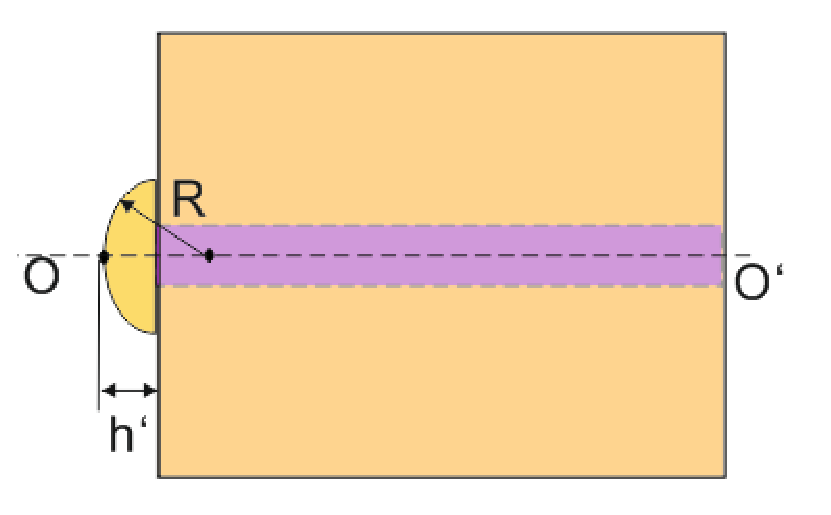
\includegraphics[width=0.7\textwidth]{bilder/lensed_waveguide}
\caption{Schema of a lensed buried waveguide.}
\label{fig:lensed_waveguide}
\end{figure}

\subsection{Coupling between TLF and regular buried waveguide}
\label{sect:optim_lensed_regular}
%basic_buried_waveguide
\begin{figure}[!ht]
\centering
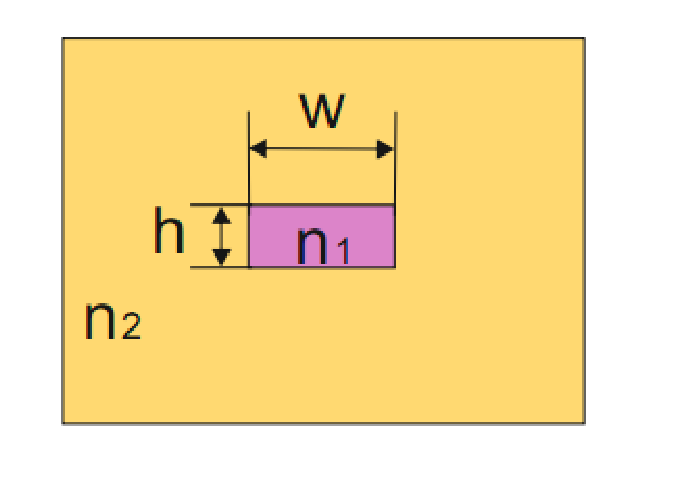
\includegraphics[width=0.6\textwidth]{bilder/buried_waveguide}
\caption{Schema of a basic buried waveguide.}
\label{fig:buried_waveguide}
\end{figure}
In agreement with the waveguide in the experiment, the buried waveguide model like Fig. \ref{fig:buried_waveguide} in this section obtains the identical dimensions ($w01\mu$m and $h00.5\mu$m) and refractive indexes (n$_{1}$ and n$_{2}$) with the original waveguide.\\ 
Fig. \ref{fig:curve_coupling_basic_buried_waveguide} shows the coupling efficiency between TLF and the regular buried waveguide due to the frequencies. The coupling efficiency at the working frequency $282$THz reaches about $51.3\%$, which is relative higher than that of the stripped rib waveguide. This value will be referred for further discussion about coupling from TLF to the lensed waveguide.  
\begin{figure}[!ht]
\centering
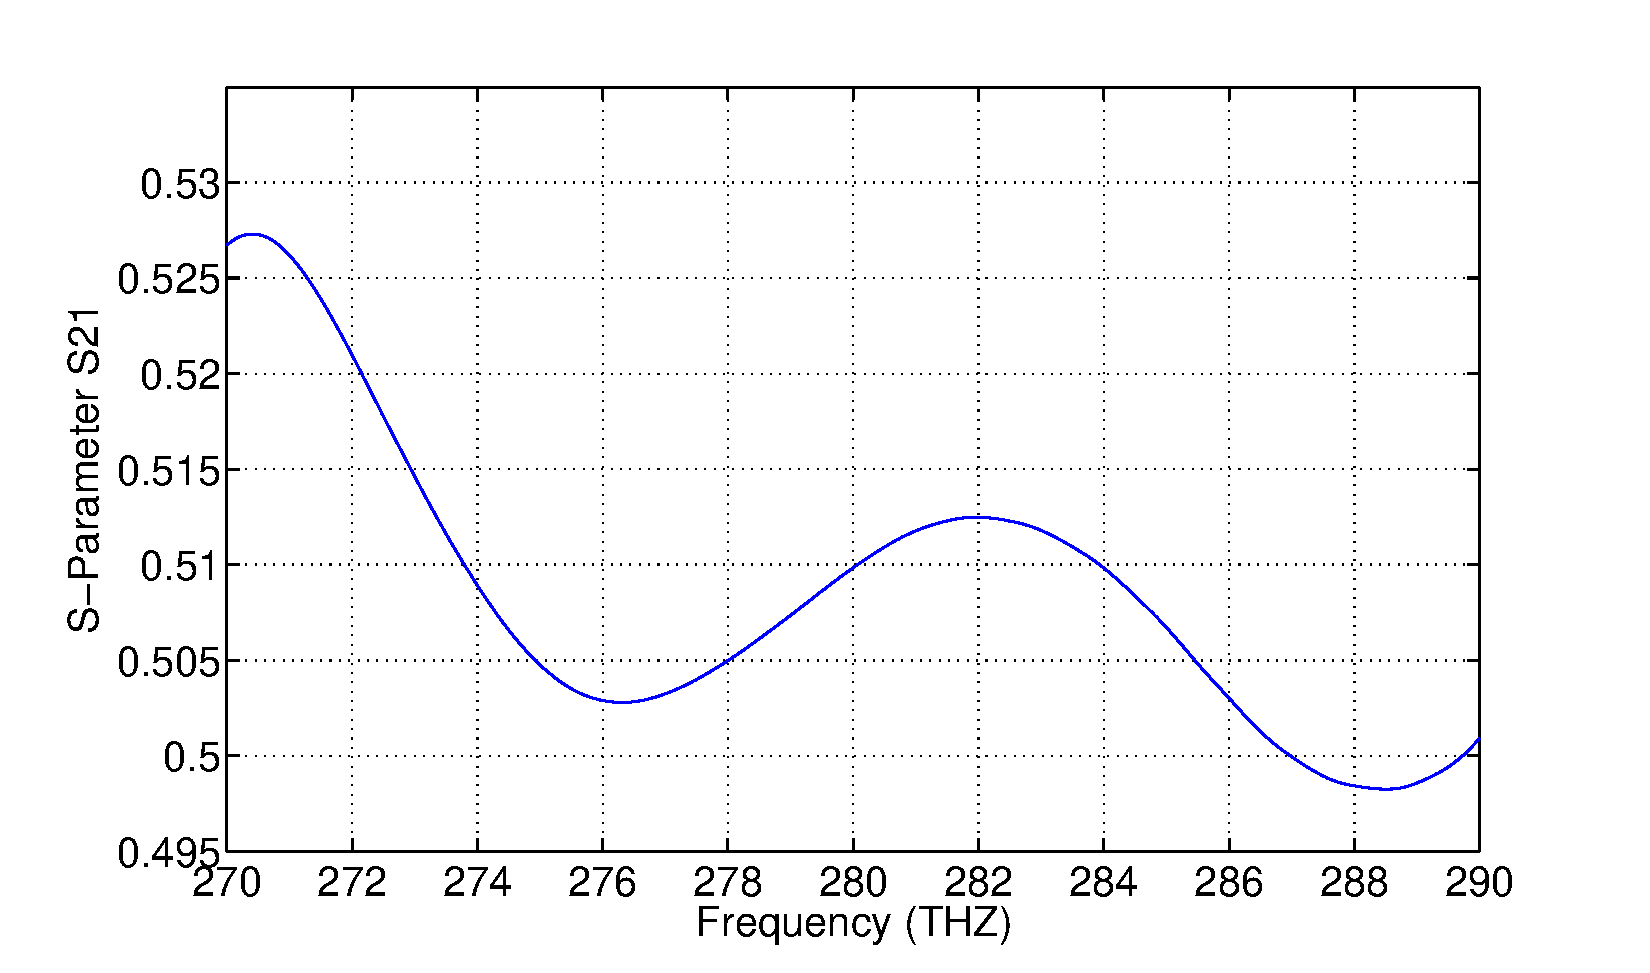
\includegraphics[width=0.8\textwidth]{bilder/s21_sym_waveguide}
\caption{Coupling efficiency curve between TLF and the basic buried waveguide due to frequency domain.}
\label{fig:curve_coupling_basic_buried_waveguide}
\end{figure}


\subsection{Effect of lens height}

In this section we aim to find out the geometric effect of lensed waveguide, whose lens is made from the same material with the substrate. Here we are going to change the lens property height with a constant lens radium. In Tab. \ref{tab:coupling_lensed_waveguide_height} the coupling efficiency for these arrangements are collected. The results can also be presented as Fig. \ref{fig:coupling_lenses_curve_hxx}, from which the coupling behaviors between TLF and lensed waveguide    
\begin{table}
\caption{Cupling efficiency between TLF and lensed waveguide due to changing the lens height}
\centering
\begin{tabular}{|c|c|c|c|}
\hline
\multirow{2}{*}{Height($\mu$m)}&\multicolumn{3}{c|}{Radium($\mu$m)}\\
\cline{2-4}
 			&	2&	2.5&	3\\
\hline
$0.4$&$54\%$&$53.4\%$&$52.9\%$\\
$0.6$&$58.35\%$&$57.4\%$&$56.9\%$\\
$0.8$&$57.3\%$&$56.7\%$&$56.3\%$\\
$1.0$&$60\%$&$58.8\%$&$57.8\%$\\
$1.2$&$60.7\%$&$59.1\%$&$57.9\%$\\
$1.4$&$61.7\%$&$59.9\%$&$58.8\%$\\
$1.6$&$65.1\%$&$62.7\%$&$60.7\%$\\
$1.8$&$62.9\%$&$60.9\%$&$59.9\%$\\
$2.0$&$69\%$  &  $66\%$&$63\%$\\
$2.2$&--------&$62.5\%$&$61.6\%$\\
$2.4$&--------&$68.8\%$&$64.4\%$\\
$2.6$&--------&--------&$66.7\%$\\
$2.8$&--------&--------&$64.8\%$\\
$3.0$&--------&--------&$68.9\%$\\
\hline

\end{tabular}
\label{tab:coupling_lensed_waveguide_height}
\end{table}
Compare these values with that of the coupling between TLF and basic buried waveguide, a proper designed micro lens on the waveguide can greatly improve the coupling efficiency. And it can also be found from Fig. \ref{fig:coupling_lenses_curve_hxx} that for a fix radium the most efficient lens configuration exist at the highest lens height or a hemisphere lens. But an exact hemisphere structure (height$=2\mu$m,Radium$=2\mu$m) may be not so easy for fabrication. Therefore the second efficient configuration (height$=1.6\mu$m,Radium$=2\mu$m) must be  an optimal option among simulations. 
\begin{figure}[!ht]
\centering
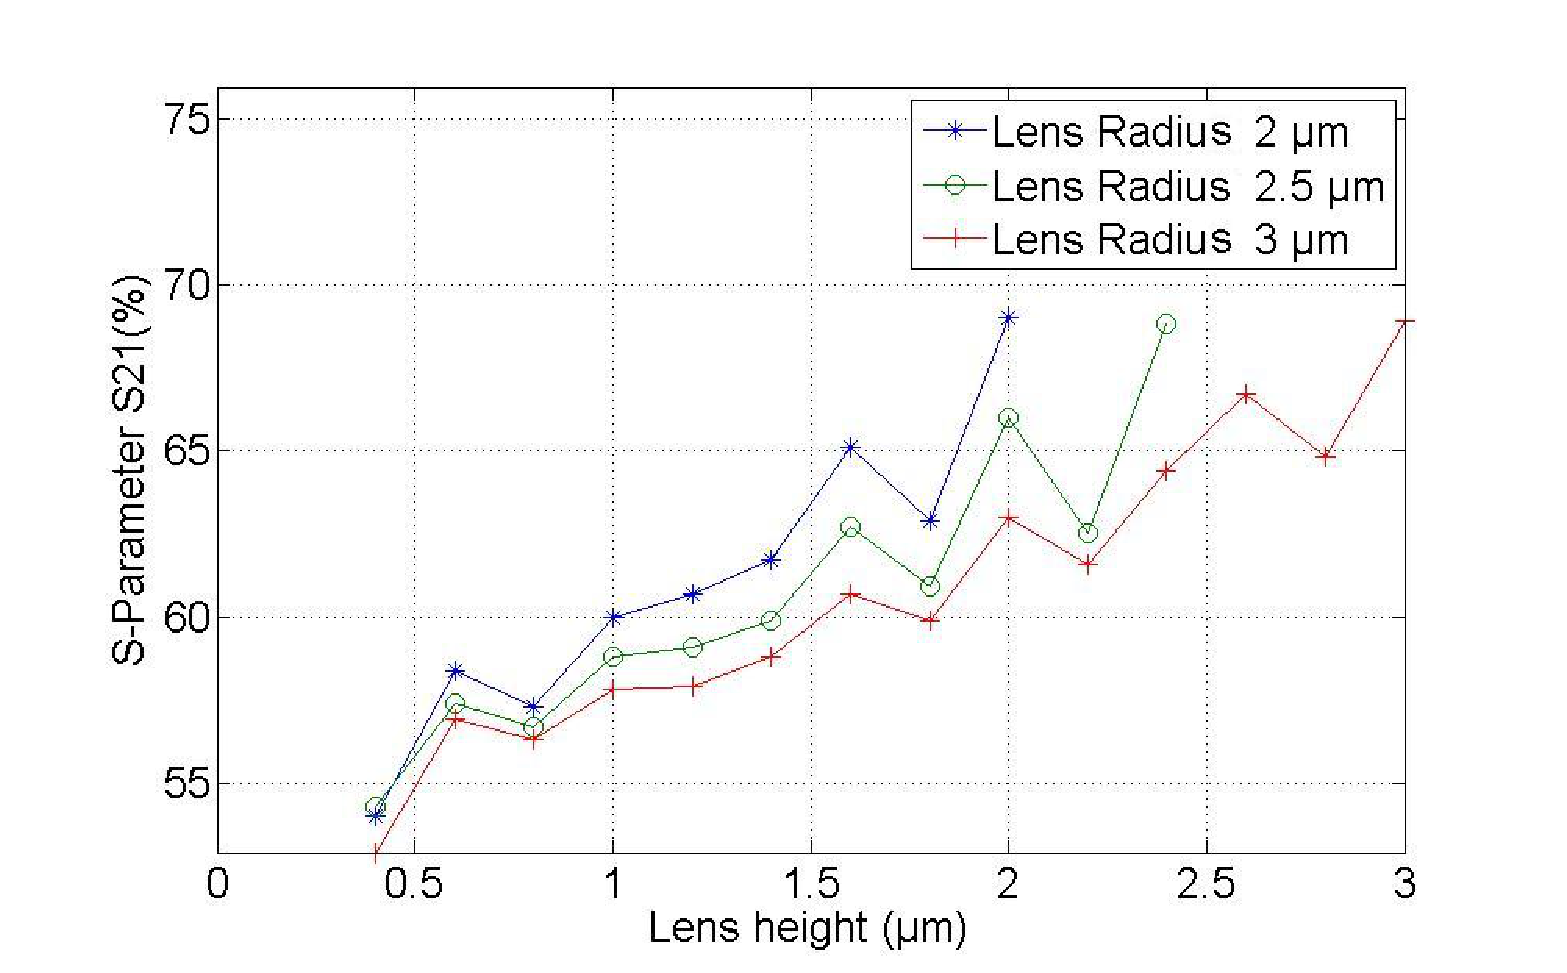
\includegraphics[width=0.8\textwidth]{bilder/s21_fix_lens_radium_hxx}
\caption{Coupling efficiency due to the variation of the lens height.}
\label{fig:coupling_lenses_curve_hxx}
\end{figure}

The reason of the efficiency change can be explained by Fig.  \ref{fig:matlab_coupling_lenses_rxx}-\ref{fig:matlab_coupling_lenses_rxx2}. From the former cure Fig. \ref{fig:matlab_coupling_lenses_rxx} we can tell that beam spot size at the working distance is bigger than the dimensions of the waveguide interface and from Fig. \ref{fig:matlab_coupling_lenses_rxx2} we understand the reason because rays near margin are penetrating mostly into substrate. In Fig. \ref{fig:matlab_coupling_lenses_rxx} rays near margin are refracted and focused to axis, so that the beam spot size is decreased and more rays are concentrated into waveguide to make the coupling become more adaptable.\\   
\begin{figure}[!ht]
\centering
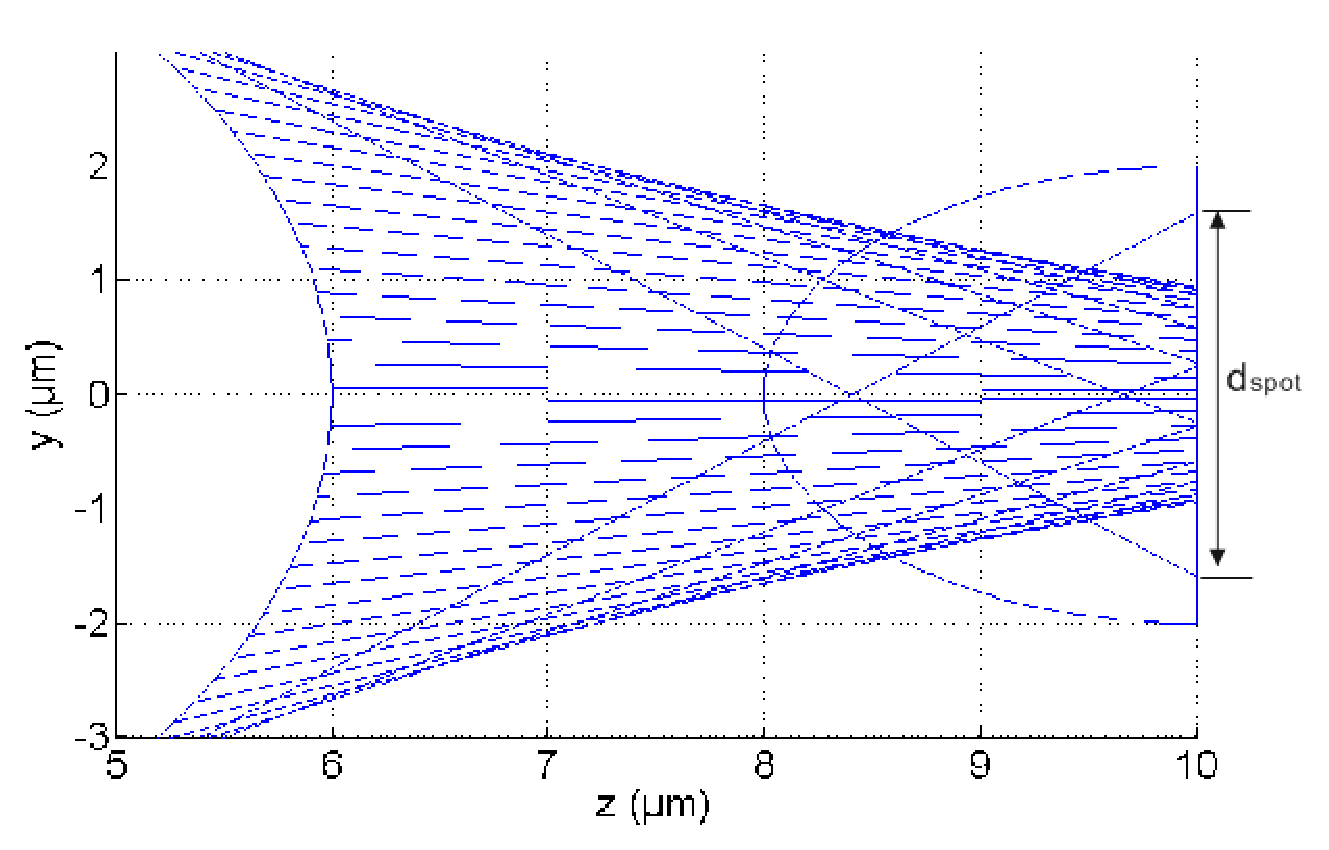
\includegraphics[width=0.8\textwidth]{bilder/beam_ray_without_refract}
\caption{The marginal rays propagate without refraction.}
\label{fig:matlab_coupling_lenses_rxx}
\end{figure}
\begin{figure}[!ht]
\centering
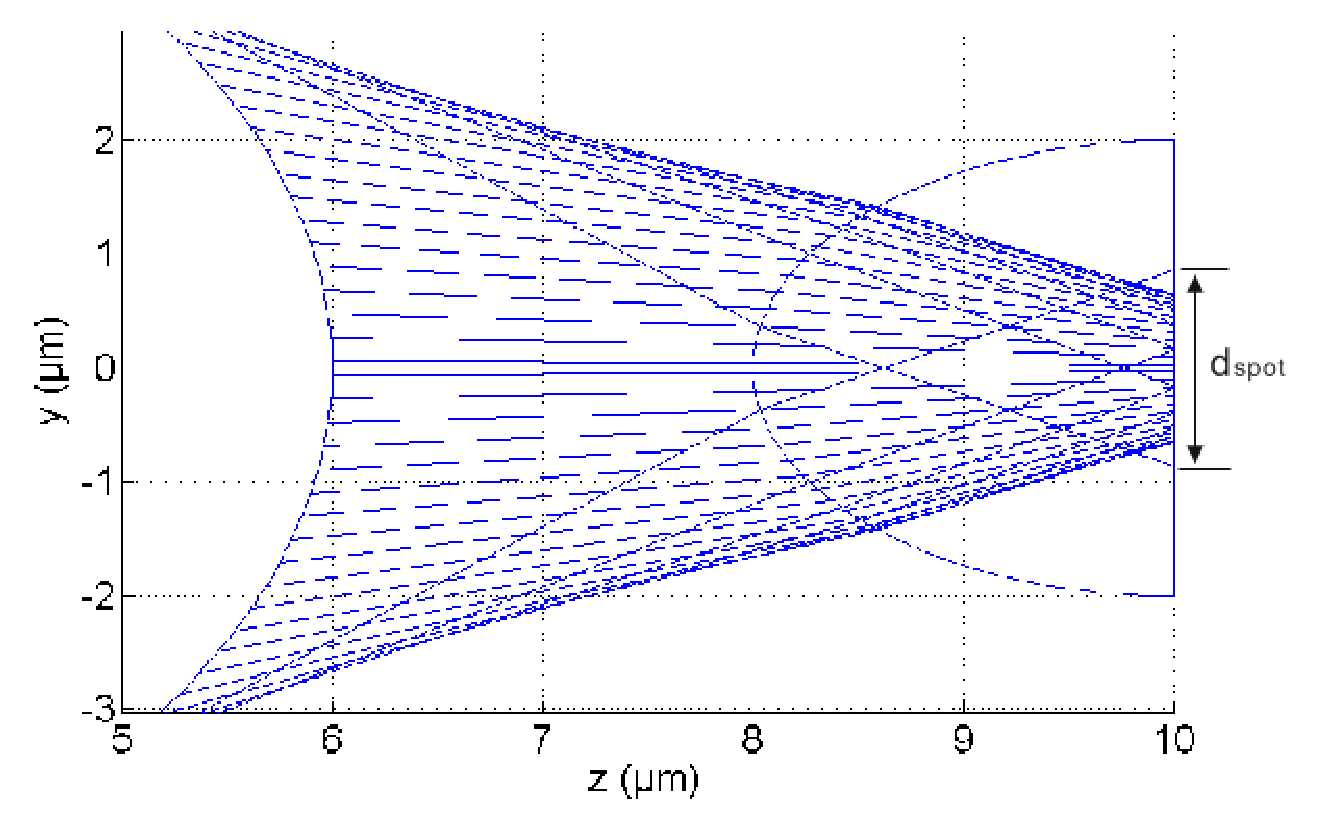
\includegraphics[width=0.8\textwidth]{bilder/beam_ray_refract}
\caption{The marginal rays are concentrated by lens of the waveguide.}
\label{fig:matlab_coupling_lenses_rxx2}
\end{figure}
For more information about the spot size of this configuration we can draw the Fig. \ref{fig:lensed_guide_spot_size_curve}. And the spot sizes changing agree well with the corresponding coupling efficiency.
\begin{figure}[!ht]
\centering
\includegraphics[width=0.8\textwidth]{bilder/spot_fix_lens_radium_hxx}
\caption{The spot size curve at lensed waveguide interface due to changing lens height}
\label{fig:lensed_guide_spot_size_curve}
\end{figure}

%
\subsection{Effect of lens radius}
%\subsection{Effect of lens radium}
%lensed_waveguide_radium
In this part we are going to fixed height of the lens on the waveguide and change the lens radium.
In Tab. \ref{tab:coupling_lensed_waveguide_radium} the lens height is choosed for $1\mu$m, $1.5\mu$m and $2\mu$m respectively. Change the lens radium from $2\mu$m to $3.6\mu$m and observe $|S21|$ as coupling efficiency.

\begin{table}
\caption{Cupling efficiency between TLF and lensed waveguide due to changing the lens radium}
\centering
\begin{tabular}{|c|c|c|c|c|}
\hline
\multicolumn{2}{|c}{}&\multicolumn{3}{c|}{Height($\mu$m)}\\
\hline
\multicolumn{2}{|c|}{}&	1&	1.5&2\\
\hline
\multirow{6}{*}{Radium($\mu$m)}&$2.0$& $59.5\%$	&$61.3\%$	&$69\%$\\
&$2.2$& $59\%$		&$60.8\%$	&$68.3\%$\\
&$2.4$&$59\%$		&$60.3\%$	&$66.8\%$\\
&$2.6$&$58.6\%$	&$59.9\%$	&$65.3\%$\\
&$2.8$&$58.2\%$	&$59.3\%$	&$64\%$\\
&$3.0$&$57.8\%$	&$58.7\%$	&$63\%$\\
\hline
\end{tabular}
\label{tab:coupling_lensed_waveguide_radium}
\end{table}

According above data the coupling behavior curve can be mapped in Fig. \ref{fig:coupling_lenses_curve_rxx}. Apparently it can be told that the coupling efficiencies under different lens heights are monotonously declining due to the variation of the lens radium.
\begin{figure}[!ht]
\centering
\includegraphics[width=0.8\textwidth]{bilder/s21_fix_lens_height_rxx}
\caption{Coupling efficiency due to changing the lens radium}
\label{fig:coupling_lenses_curve_rxx}
\end{figure}

And the spot size curve in Fig. \ref{fig:lensed_guide_spot_size_curve_rxx} along the variation of the lens radium behave inversely in compare with the trends of coupling efficiency.
\begin{figure}[!ht]
\centering
\includegraphics[width=0.8\textwidth]{bilder/spot_fix_lens_height_rxx}
\caption{The spot size curve at lensed waveguide interface due to changing lens height}
\label{fig:lensed_guide_spot_size_curve_rxx}
\end{figure}


\subsection{Extension of lensed waveguides}
\label{sect:optim_lensed_ext}
%Subsection{extension}
%lensed_waveguide_extension
From \cite{integrated_coupling_between_LD_SMF} we can find more ideas to promote the coupling efficiency between TLF and lensed waveguide. The author at the end has presented a tapered core fiber, with which the core is capable to confine more beam rays. And we also get to know there is a small distance between the lens end and core interface because the lens end may not be the minimum spot location for a lensed waveguide. Thus is it possible to gain higher coupling efficiency by expanding properly the distance between the lens and the core within the lensed waveguide.

%
\chapter{Conclusion}
%conclusion

%description of the project and theory.
%description of the project and theory.
Coupling the light from optical fiber to photonic waveguide (fiber-to-chip) is a common topic for research and application in optical communication. As the light source the normal fiber has a generally an interface bigger than the dimension of the photonic waveguide. In order to promote the coupling efficiency the tapered lensed fibers (TLF) are usually applied as the light source. Thus the coupling between TLF and photonic waveguide becomes an attractive agenda of the optic research. \\ 

%purpose of this work
This work aims for the optimal solution for the effective coupling between TLF and photonic waveguide. In order to achieve this goal the coupling models have been constructed and simulated with the aid of CST MWS. In this work the modelling procedure and the analyses of the result are recounted.\\

%the content and the result of this work
%summary of each chapter, 
In chapter. \ref{chp:background} the basic knowledge about the geometric optic, fiber optic, Gaussian beam, finite integration technigue and S-Parameter is listed. The above knowledge could be helpful to understand some terms of this work. The chapter. \ref{chp:model} gives readers of this work at first an impression about the technical details of the experimental objects. Then the modelling procedure, how the model is simplified and how the properties of models look like, is introduced. Especially, two types of TLF models are compared and one is finally chosen for the further discussion. In chapter. \ref{chp:optim} simulations about the effective coupling between TLF and the waveguide is divided into five parts. In the first part, the simulation aims at the effect of displacing the waveguide on the coupling efficiency. In the second part we try the same coupling configuration in oil environment instead of in air. In the third part the effect of the refractive index is discussed. After that, the fourth and fifth parts provide two important techniques of waveguide interface, tapered and lensed interface, for promoting the coupling ability.\\        
 
%compare and conclude the results, advice for experiment 
According to the results from all simulations in this work, a good designed waveguide interface can greatly affect the coupling ability of Fiber-to-Chip. The original coupling arrangement in this work achieved an efficiency $48.9\%$. The waveguide with $n=1.8$ in coupling leads to an attractive result $62.5\%$. The simply constructed tapered interface gained maximally a value about $54\%$. In comparison to the tapered interface, lensed interface of the waveguide can catch the efficiency about $69\%$ in this work. From this view, the lensed interface is the most optimal option for Fiber-to-Chip coupling. But coupling ability is not the exclusive aspect for the practical application. The fabrication cost must be considered. The method of using simple tapered interface or using another guide material is easier for the fabrication than the lensed interface. Thus the simple tapered interface is a more economical solution. \\
       
% the extensions of this work.
There are more and more interesting designs for the effective Fiber-to-Chip coupling. The tapered plasmonic waveguide in \cite{tapered_plasmonic_waveguides} is the application of SPP mode wave provided by metal/dielectric interface. This design is cutoff free and SPP field in it can be highly concentrated. Alonso-Ramos involve grating as coupler in \cite{fiber_to_chip_grating_waveguides} to extract beams into another planar waveguide. In his developments he reached the coupling efficiency of $65.6\%$. Besides above two designs section \ref{sect:optim_tapered_ext} and section \ref{sect:optim_lensed_ext} of this work also mention two extension for further development. The hybrid tapered interface and lensed interface with a neck are properly uneasy for fabrication, but as a simulation project they can still engage our attention.









%\input{mainmatter/Chapter_optimize/tab_test}



